% Hier beginnt der Code für das Kapitel Trigonometrische Funktionen.
% Annahme: Alle Pakete und Definitionen aus dem Hauptdokument (math_learning_material_v2) 
% sind hier gültig und werden im Hauptdokument geladen.

\section{Trigonometrische Funktionen – Die Mathematik der Schwingungen und Wellen}
\label{sec:trigonometrische_funktionen}

Nachdem wir uns mit Polynomen, Exponential- und Logarithmusfunktionen beschäftigt haben, wenden wir uns nun einer weiteren wichtigen Funktionsklasse zu: den \textbf{trigonometrischen Funktionen}. Die bekanntesten Vertreter sind \textbf{Sinus ($\sin x$)}, \textbf{Kosinus ($\cos x$)} und \textbf{Tangens ($\tan x$)}.

\begin{tcolorbox}[colback=blue!5!white, colframe=blue!75!black, title=Was du in diesem Kapitel lernen wirst:]
Nachdem du dieses Kapitel durchgearbeitet hast, wirst du in der Lage sein:
\begin{itemize}[noitemsep, topsep=0pt, leftmargin=*, itemsep=2pt]
    \item die Bedeutung des \textbf{Bogenmaßes} für Winkel zu verstehen und es sicher im Zusammenhang mit trigonometrischen Funktionen anzuwenden sowie zwischen Grad- und Bogenmaß umzurechnen.
    \item die Funktionen \textbf{Sinus ($\sin x$)} und \textbf{Kosinus ($\cos x$)} am Einheitskreis zu definieren und ihre grundlegenden Eigenschaften (Definitions- und Wertebereich, Periode $2\pi$, Nullstellen, Extremstellen, Symmetrie) sowie den trigonometrischen Pythagoras ($\sin^2x + \cos^2x = 1$) zu kennen und zu nutzen.
    \item die \textbf{Tangensfunktion ($\tan x$)} als Quotient aus Sinus und Kosinus zu definieren und ihre wesentlichen Eigenschaften (Definitionsbereich mit Polstellen, Wertebereich, Periode $\pi$, Nullstellen, Symmetrie) zu beschreiben.
    \item die \textbf{Ableitungen} der Grundfunktionen $(\sin x)' = \cos x$, $(\cos x)' = -\sin x$ und $(\tan x)' = \frac{1}{\cos^2 x} = 1+\tan^2x$ zu kennen und anzuwenden.
    \item die grundlegenden \textbf{Stammfunktionen} $\int \cos x \,dx = \sin x + C$ und $\int \sin x \,dx = -\cos x + C$ zu bilden und für einfache bestimmte Integrale zu nutzen.
    \item \textbf{transformierte Sinus- und Kosinusfunktionen} der Form $f(x) = A \sin(B(x-C)) + D$ zu analysieren, indem du die Bedeutung der Parameter für Amplitude, Periode, Phasen- und y-Verschiebung interpretierst, und solche Funktionen zu skizzieren oder aus Graphen abzuleiten.
    \item die allgemeinen \textbf{Ableitungsregeln} (Produkt-, Quotienten- und Kettenregel) sicher auf Funktionen anzuwenden, die trigonometrische Terme enthalten (oft in Kombination mit Polynomen oder Exponentialfunktionen).
    \item eine vollständige \textbf{Kurvendiskussion} für Funktionen mit trigonometrischen Anteilen durchzuführen, um deren Graphen und charakteristische Merkmale zu analysieren.
    \item die fundamentale Rolle trigonometrischer Funktionen bei der Modellierung \textbf{periodischer Vorgänge} und Schwingungen zu verstehen.
\end{itemize}
Du wirst somit die Mathematik der Wellen und Zyklen meistern und dein Repertoire an analysierbaren Funktionen entscheidend erweitern!
\end{tcolorbox}
\bigskip

Diese Funktionen sind unerlässlich, um \textbf{periodische Vorgänge} zu beschreiben – also Phänomene, die sich in regelmäßigen Abständen wiederholen. Denk zum Beispiel an:
\begin{itemize}
    \item Schwingungen eines Pendels oder einer Gitarrensaite.
    \item Wellenbewegungen wie Wasserwellen oder Schallwellen.
    \item Kreisbewegungen, z.B. die Position eines Punktes auf einem sich drehenden Rad.
    \item Jahreszeitliche Schwankungen von Temperaturen oder Tageslängen.
    \item Wechselstrom in der Elektrotechnik.
\end{itemize}
Die trigonometrischen Funktionen sind die mathematische Sprache, um diese periodischen Muster präzise zu erfassen und zu analysieren.

\begin{infoboxumgebung}{Winkel im Bogenmaß – Die 'natürliche' Einheit für Winkel}
In der höheren Mathematik und besonders bei der Analysis von trigonometrischen Funktionen werden Winkel fast ausschließlich im \textbf{Bogenmaß} (Radiant, abgekürzt rad) angegeben, nicht im Gradmaß (z.B. $30^\circ, 90^\circ, 360^\circ$).
\textbf{Was ist das Bogenmaß?}
Stell dir einen Kreis mit Radius $r=1$ vor (den Einheitskreis). Das Bogenmaß eines Winkels $\alpha$ ist die Länge des Kreisbogens, den dieser Winkel auf dem Einheitskreis 'ausschneidet'.
\begin{itemize}
    \item Ein Vollkreis hat $360^\circ$. Der Umfang des Einheitskreises ist $U = 2\pi r = 2\pi \cdot 1 = 2\pi$.
    Also entspricht $360^\circ$ einem Bogenmaß von $2\pi$.
    \item Daraus folgt: $180^\circ \widehat{=} \pi \text{ rad}$
    \item $90^\circ \widehat{=} \frac{\pi}{2} \text{ rad}$
    \item $60^\circ \widehat{=} \frac{\pi}{3} \text{ rad}$
    \item $45^\circ \widehat{=} \frac{\pi}{4} \text{ rad}$
    \item $30^\circ \widehat{=} \frac{\pi}{6} \text{ rad}$
\end{itemize}
\textbf{Umrechnung:}
\begin{itemize}
    \item Gradmaß in Bogenmaß: $\text{Bogenmaß} = \text{Gradmaß} \cdot \frac{\pi}{180^\circ}$
    \item Bogenmaß in Gradmaß: $\text{Gradmaß} = \text{Bogenmaß} \cdot \frac{180^\circ}{\pi}$
\end{itemize}
Wenn bei trigonometrischen Funktionen keine Einheit angegeben ist (z.B. $\sin(2)$), ist immer das Bogenmaß gemeint! Die Ableitungsregeln, die wir kennenlernen werden, gelten nur, wenn der Winkel im Bogenmaß gegeben ist.
\end{infoboxumgebung}

\subsection{Sinus ($\sin x$) und Kosinus ($\cos x$) – Die Grundpfeiler}
\label{subsec:sinus_kosinus_grundlagen}

Die Funktionen $f(x)=\sin(x)$ und $g(x)=\cos(x)$ sind die fundamentalsten trigonometrischen Funktionen.

\subsubsection{Geometrische Bedeutung am Einheitskreis}
Eine anschauliche Definition von Sinus und Kosinus erhält man am \textbf{Einheitskreis} (Kreis mit Radius $r=1$ um den Ursprung eines Koordinatensystems).
Betrachtet man einen Winkel $\alpha$ (im Bogenmaß), der von der positiven x-Achse gegen den Uhrzeigersinn gemessen wird, so schneidet der freie Schenkel des Winkels den Einheitskreis in einem Punkt $P(x_P|y_P)$. Dann gilt:
\begin{itemize}
    \item $\cos(\alpha) = x_P$ (die x-Koordinate des Punktes $P$)
    \item $\sin(\alpha) = y_P$ (die y-Koordinate des Punktes $P$)
\end{itemize}
\begin{center}
    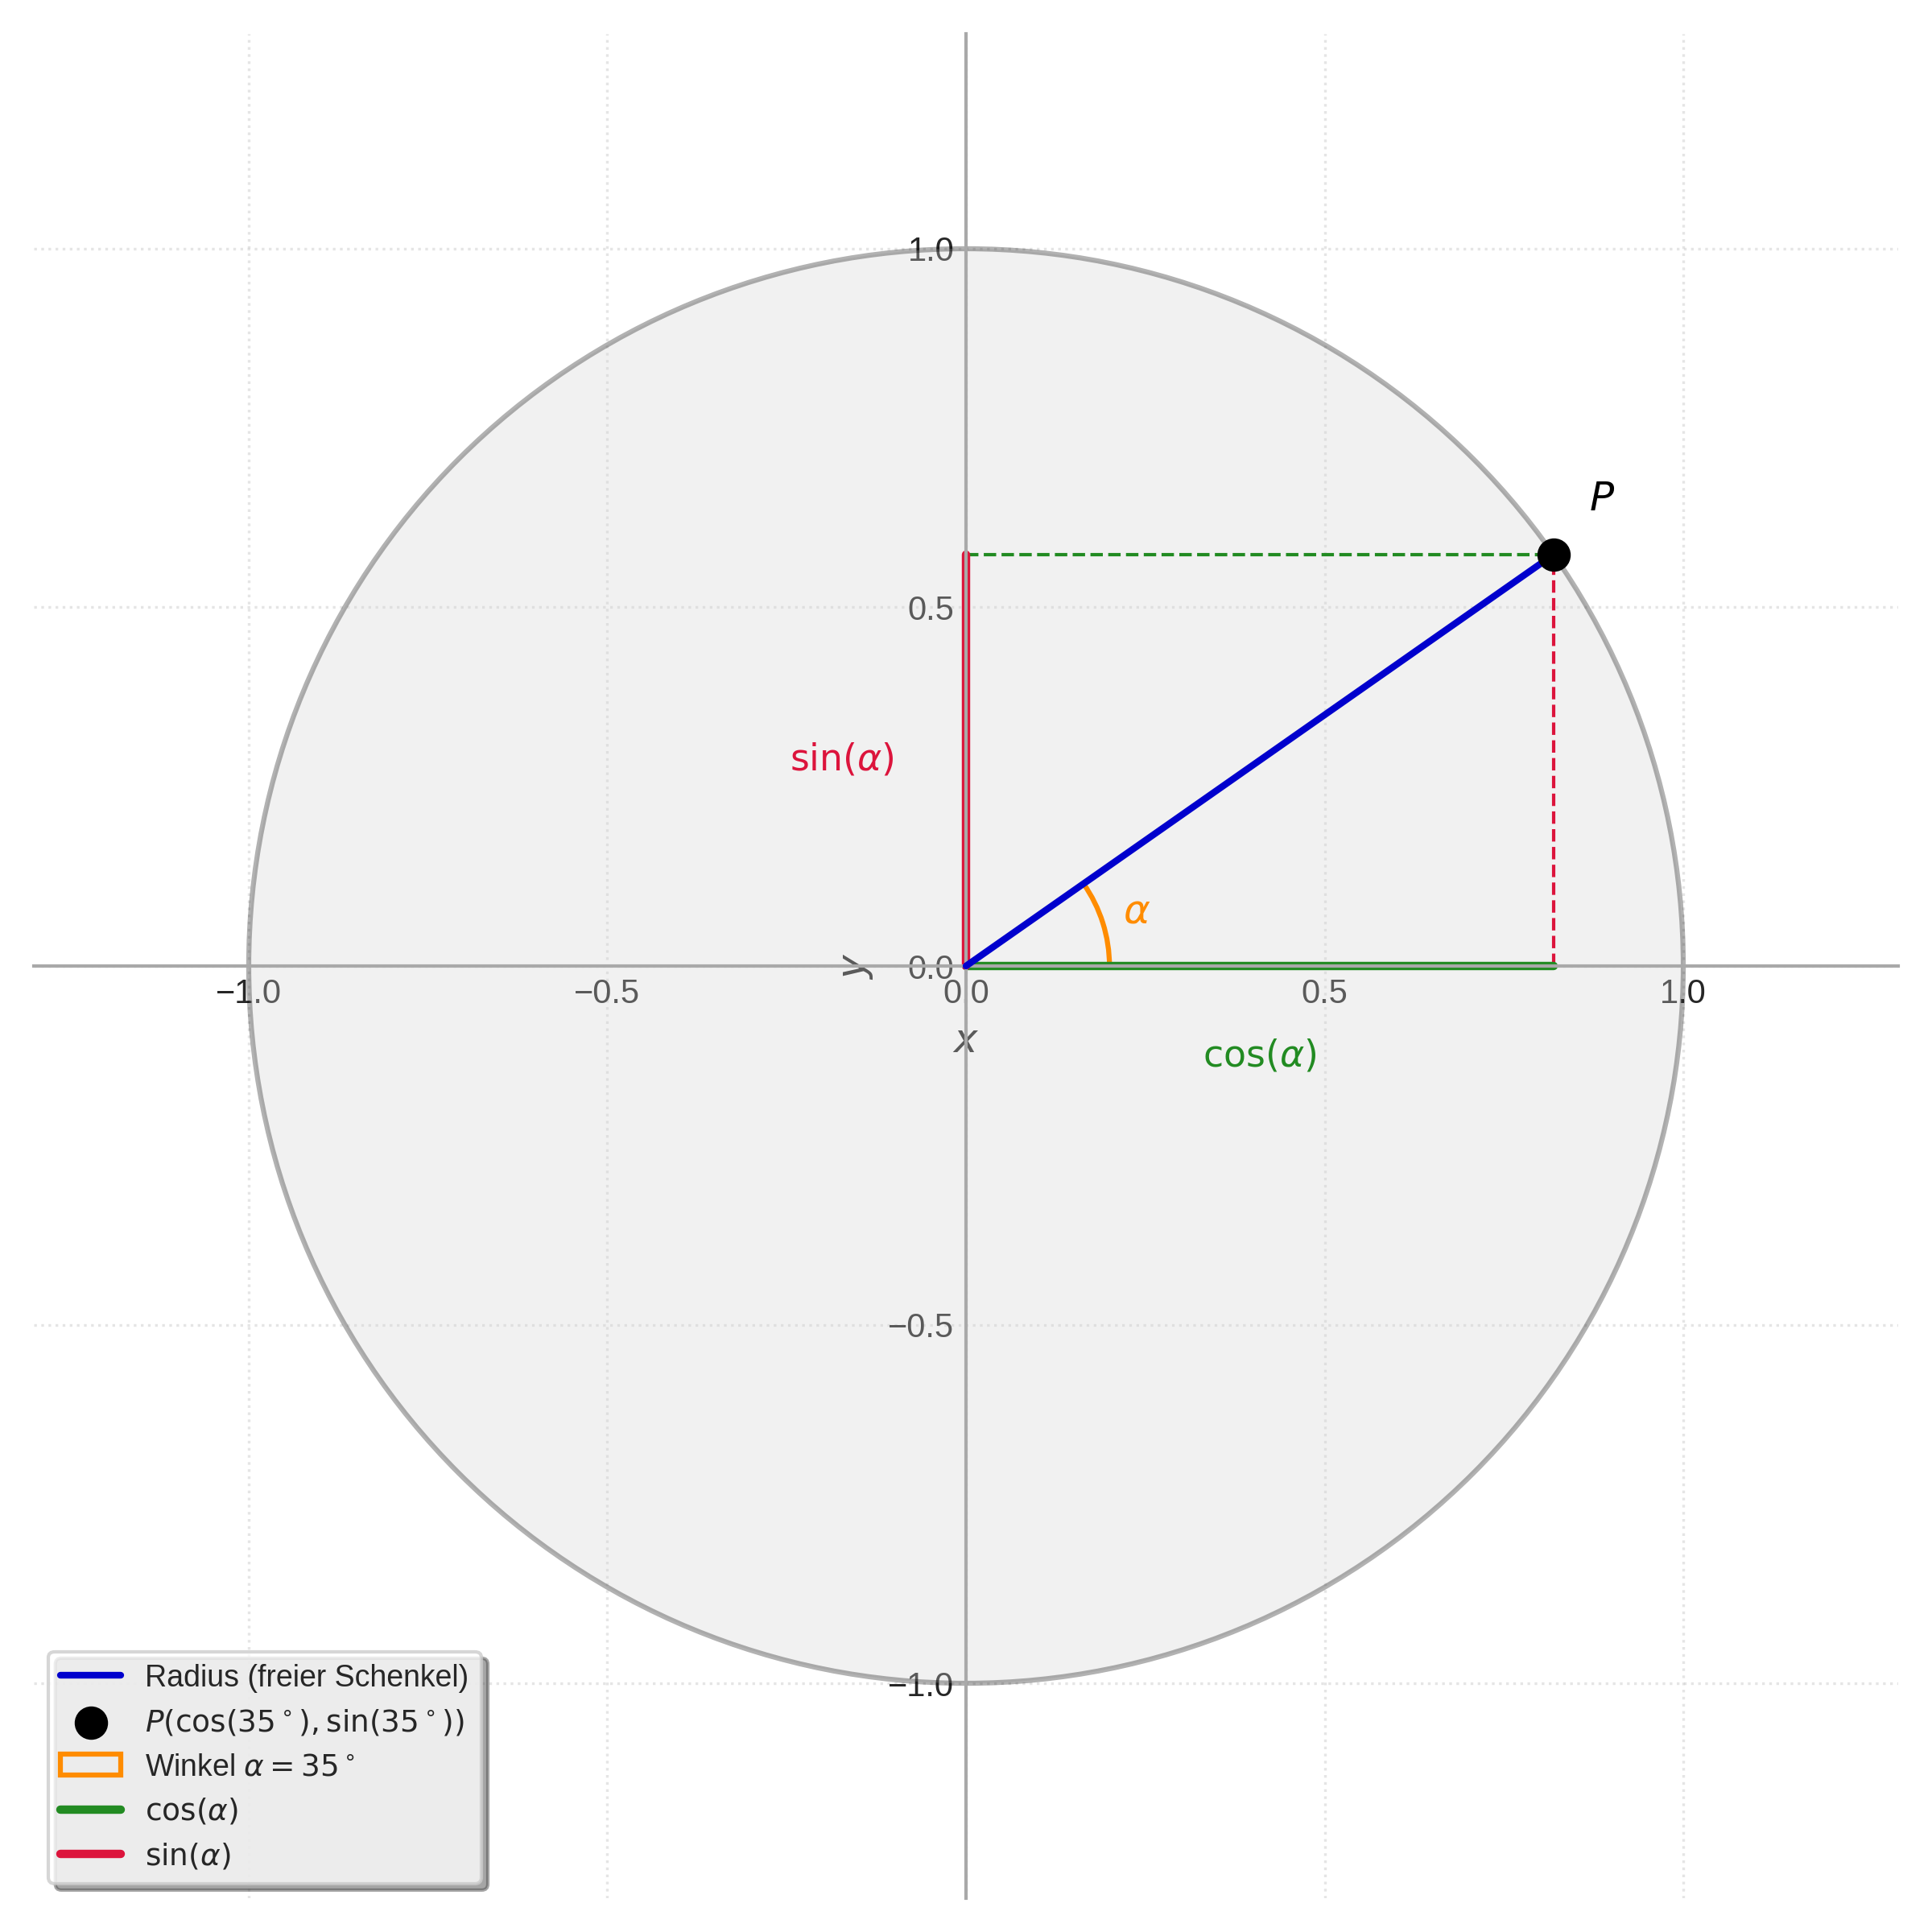
\includegraphics[width=0.7\textwidth]{grafiken/Trig_Einheitskreis.png}
    \captionof{figure}{Definition von Sinus und Kosinus am Einheitskreis}
    \label{fig:einheitskreis}
\end{center}
Aus dieser Definition am Einheitskreis ergeben sich viele wichtige Eigenschaften.

\subsubsection{Graphen und Eigenschaften von $\sin(x)$ und $\cos(x)$}

\begin{merksatzumgebung}{Eigenschaften von $f(x)=\sin(x)$ und $g(x)=\cos(x)$}
\begin{itemize}
    \item \textbf{Definitionsbereich:} $D_f = D_g = \mathbb{R}$ (man kann jeden reellen Winkel einsetzen).
    \item \textbf{Wertebereich:} $W_f = W_g = [-1, 1]$ (die Funktionswerte liegen immer zwischen -1 und 1, inklusive).
    \item \textbf{Periodizität:} Beide Funktionen sind periodisch mit der \textbf{Periode $2\pi$}. Das bedeutet, ihre Werte wiederholen sich alle $2\pi$:
        \[ \sin(x + 2\pi) = \sin(x) \quad \text{und} \quad \cos(x + 2\pi) = \cos(x) \]
    \item \textbf{Nullstellen:}
        \begin{itemize}
            \item $\sin(x) = 0$ für $x = k \cdot \pi$, wobei $k \in \mathbb{Z}$ (alle ganzen Zahlen). Also bei $x=0, \pm\pi, \pm 2\pi, \dots$
            \item $\cos(x) = 0$ für $x = \frac{\pi}{2} + k \cdot \pi$, wobei $k \in \mathbb{Z}$. Also bei $x=\pm\frac{\pi}{2}, \pm\frac{3\pi}{2}, \dots$
        \end{itemize}
    \item \textbf{Extremstellen:}
        \begin{itemize}
            \item $\sin(x)$ hat Maxima ($+1$) bei $x = \frac{\pi}{2} + 2k\pi$ und Minima ($-1$) bei $x = \frac{3\pi}{2} + 2k\pi$.
            \item $\cos(x)$ hat Maxima ($+1$) bei $x = 2k\pi$ und Minima ($-1$) bei $x = \pi + 2k\pi$.
        \end{itemize}
    \item \textbf{Symmetrie:}
        \begin{itemize}
            \item $\sin(x)$ ist \textbf{punktsymmetrisch zum Ursprung}: $\sin(-x) = -\sin(x)$.
            \item $\cos(x)$ ist \textbf{achsensymmetrisch zur y-Achse}: $\cos(-x) = \cos(x)$.
        \end{itemize}
    \item \textbf{Zusammenhang:} Die Graphen von Sinus und Kosinus sind zueinander phasenverschoben:
        $\cos(x) = \sin(x + \frac{\pi}{2})$ (Kosinus ist Sinus um $\pi/2$ nach links verschoben).
        $\sin(x) = \cos(x - \frac{\pi}{2})$ (Sinus ist Kosinus um $\pi/2$ nach rechts verschoben).
    \item \textbf{Wichtiger Grundzusammenhang (Trigonometrischer Pythagoras):} Für jeden Winkel $x$ gilt:
        \[ \sin^2(x) + \cos^2(x) = 1 \]
        (Das folgt direkt aus dem Satz des Pythagoras am Einheitskreis, da $x_P^2+y_P^2=r^2=1^2$).
\end{itemize}
\end{merksatzumgebung}

\begin{center}
    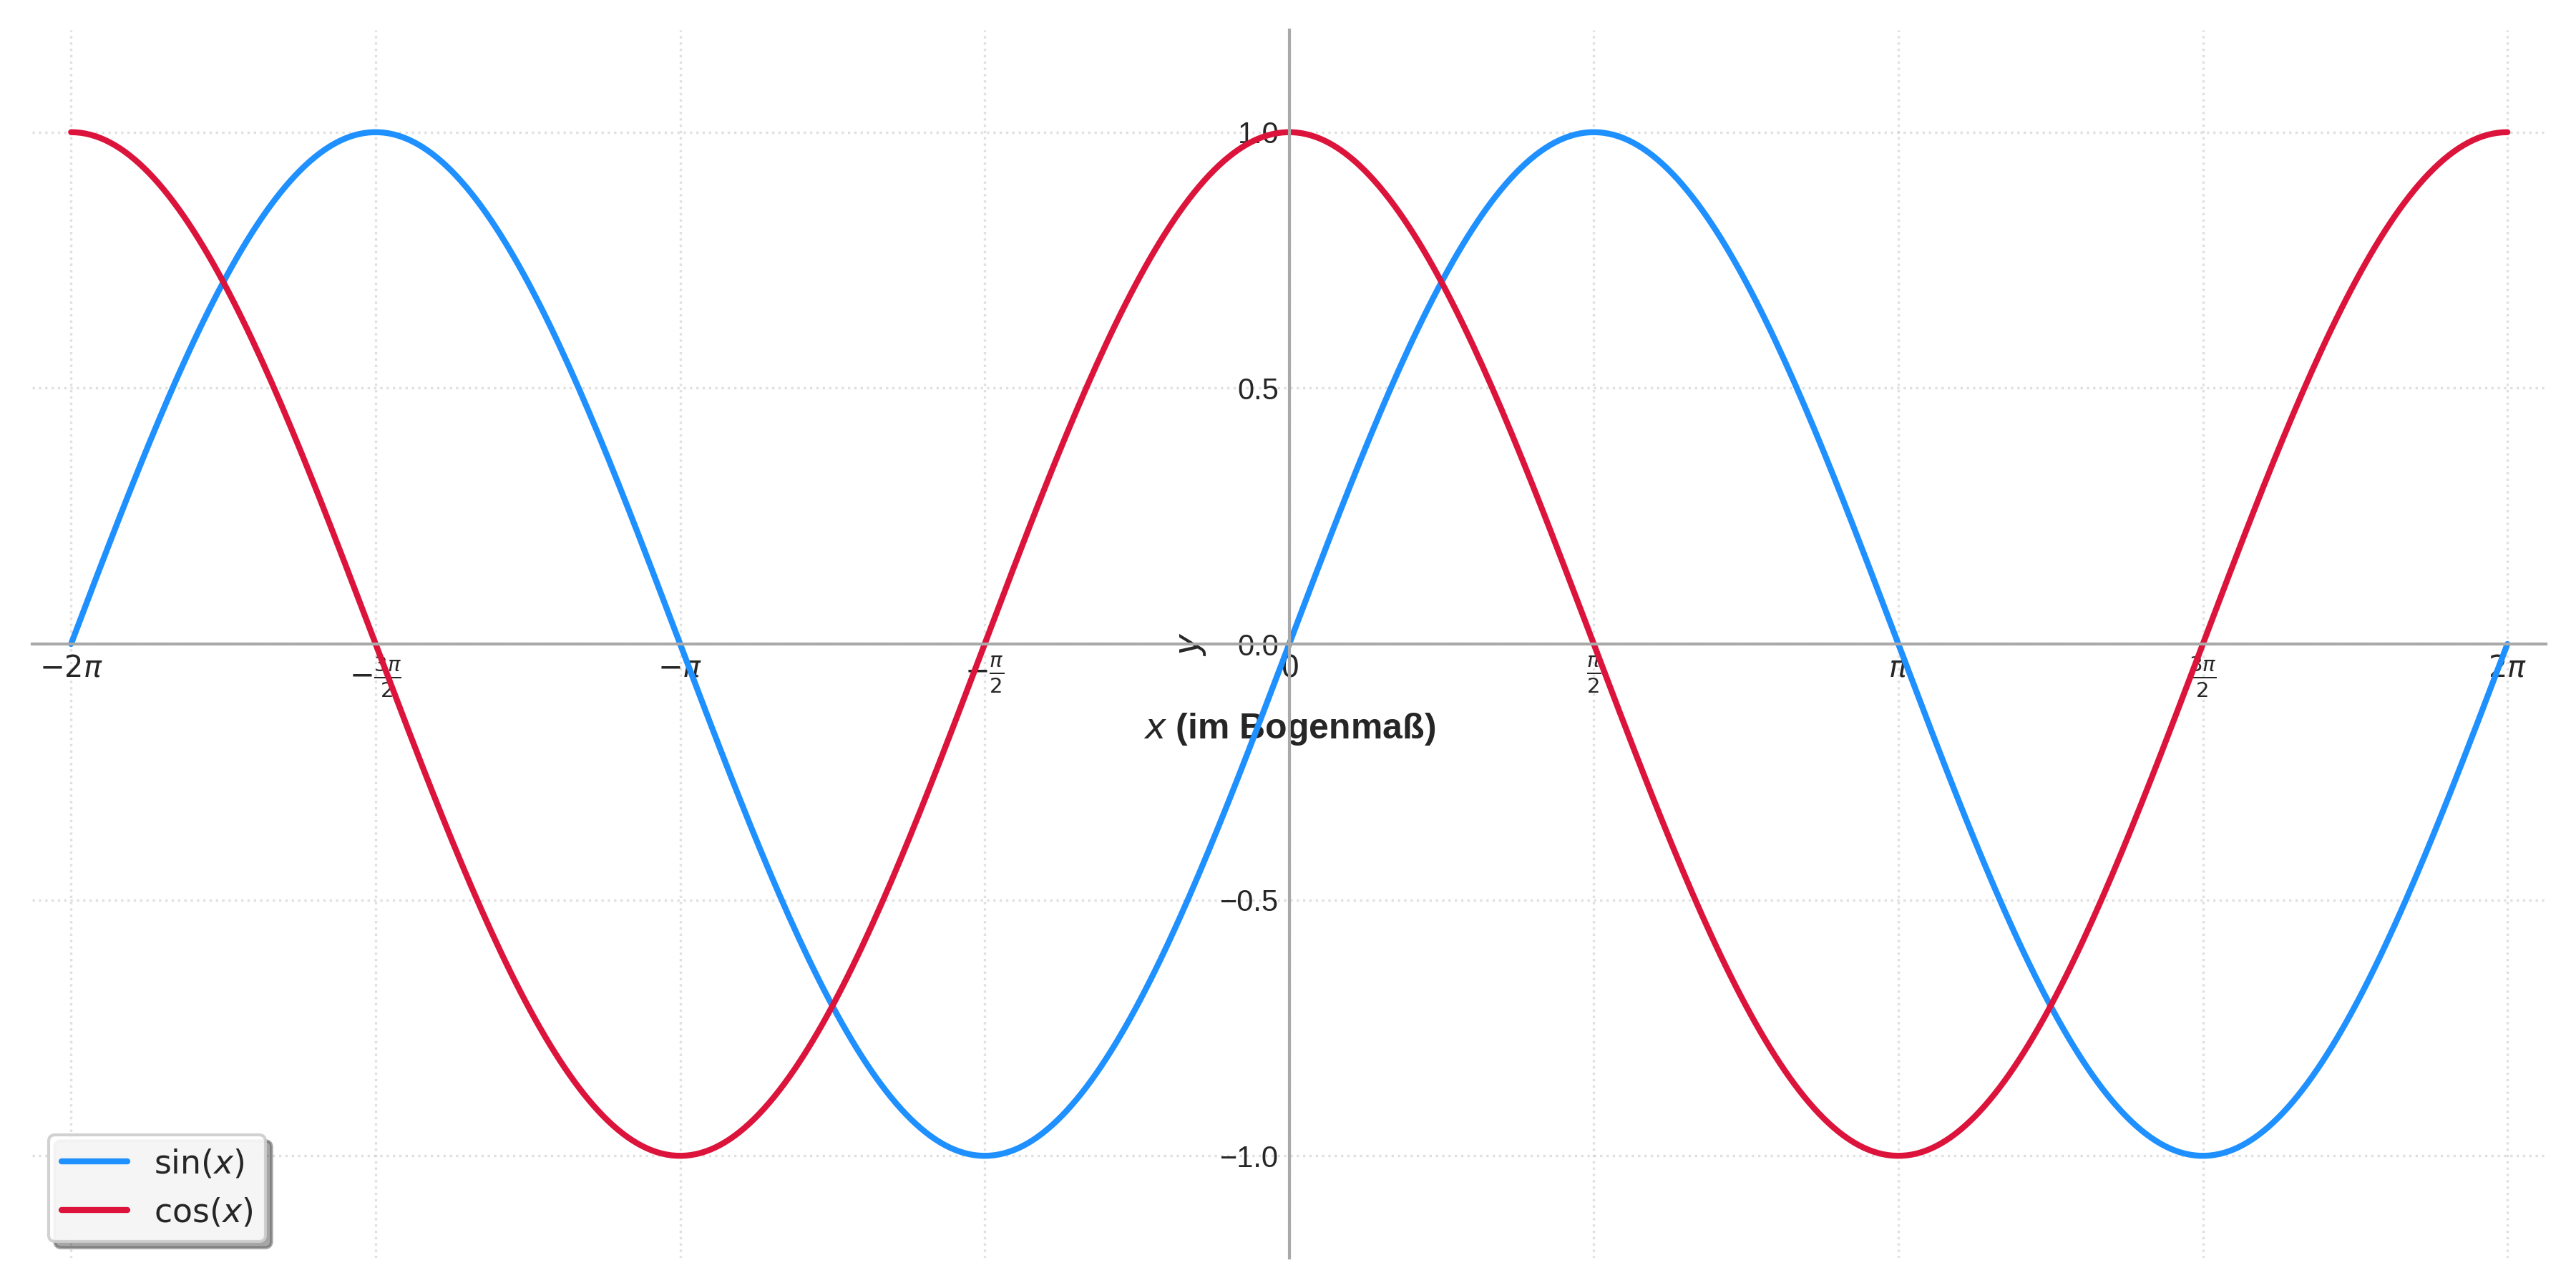
\includegraphics[width=0.9\textwidth]{grafiken/Trig_SinCos_Graphen.png}
    \captionof{figure}{Graphen der Funktionen $f(x)=\sin(x)$ und $g(x)=\cos(x)$}
    \label{fig:sincos_graphen}
\end{center}




\begin{tippumgebung}{Pythagoras im Test – Eine kleine Selbstüberprüfung}
Du hast gerade gelernt, dass für jeden Winkel $x$ gilt: $\sin^2(x) + \cos^2(x) = 1$.
Überlege einmal: Könnte es einen Winkel $x$ geben, für den gleichzeitig $\sin(x) = 0,8$ und $\cos(x) = 0,7$ gilt? Überprüfe dies, indem du die Werte in die Gleichung einsetzt. Was stellst du fest?
(Zur Erinnerung: $\sin^2(x)$ bedeutet $(\sin x)^2$.)
\end{tippumgebung}

% ... (Weiter im Text, z.B. mit der Abbildung der Sinus/Kosinus-Graphen oder dem nächsten Unterabschnitt)
\subsubsection{Ein tieferer Einblick: Sinus und Kosinus als unendliche Reihen (Taylorreihen)}
Eine faszinierende Eigenschaft vieler Funktionen in der Mathematik ist, dass sie als unendliche Summen von Potenzfunktionen dargestellt werden können – sogenannte \textbf{Taylorreihen} (oder Maclaurinreihen, wenn die Entwicklung um den Punkt $x=0$ erfolgt). Für Sinus und Kosinus sehen diese Reihen besonders elegant aus:

\begin{infoboxumgebung}{Taylorreihen für Sinus und Kosinus}
Für alle reellen Zahlen $x$ (im Bogenmaß!) gilt:
\[ \sin(x) = x - \frac{x^3}{3!} + \frac{x^5}{5!} - \frac{x^7}{7!} + \frac{x^9}{9!} - \dots = \sum_{n=0}^{\infty} (-1)^n \frac{x^{2n+1}}{(2n+1)!} \]
\[ \cos(x) = 1 - \frac{x^2}{2!} + \frac{x^4}{4!} - \frac{x^6}{6!} + \frac{x^8}{8!} - \dots = \sum_{n=0}^{\infty} (-1)^n \frac{x^{2n}}{(2n)!} \]
Dabei bedeutet $k!$ (gelesen 'k Fakultät') das Produkt aller ganzen Zahlen von 1 bis $k$: $k! = 1 \cdot 2 \cdot 3 \cdot \dots \cdot k$. (Und $0!=1$).
Zum Beispiel: $3! = 1 \cdot 2 \cdot 3 = 6$, $5! = 1 \cdot 2 \cdot 3 \cdot 4 \cdot 5 = 120$.

\textbf{Was bedeuten diese Reihen?}
\begin{itemize}
    \item Sie zeigen, dass Sinus und Kosinus im Grunde 'unendlich lange Polynome' sind.
    \item Man kann mit diesen Reihen die Werte von $\sin(x)$ und $\cos(x)$ für jedes $x$ beliebig genau annähern, indem man genügend Glieder der Summe berücksichtigt. So berechnen auch Taschenrechner diese Werte!
    \item Aus diesen Reihen lassen sich viele Eigenschaften der Funktionen ableiten, z.B. ihre Ableitungen.
\end{itemize}
Die Herleitung dieser Reihen ist fortgeschrittene Mathematik, aber ihre Existenz zu kennen, öffnet ein Fenster zu tieferen Zusammenhängen.
\end{infoboxumgebung}

\textit{Selbst-Check:} Setze $x=0$ in die Reihen für $\sin(x)$ und $\cos(x)$ ein. Was erhältst du? Vergleiche mit $\sin(0)$ und $\cos(0)$ vom Einheitskreis. (Antwort: $\sin(0)=0$, $\cos(0)=1$. Das passt!)
\begin{funfactbox}{$\pi$ aus dem Nichts? Eine unendliche Summe enthüllt die Kreiszahl!}
Die Kreiszahl $\pi \approx 3,14159\dots$ ist dir sicher bekannt. Sie beschreibt das Verhältnis des Umfangs eines Kreises zu seinem Durchmesser. Aber wie kommt man eigentlich auf diese unendlich vielen Nachkommastellen? Es gibt viele faszinierende Wege, $\pi$ zu berechnen, und einige davon haben Verbindungen zur Differential- und Integralrechnung!

Eine berühmte Methode verwendet eine unendliche Summe, die mit dem Mathematiker Gottfried Wilhelm Leibniz (einem der 'Erfinder' der Differentialrechnung) in Verbindung gebracht wird, aber auch schon früher in Indien bekannt war:
\[ \frac{\pi}{4} = 1 - \frac{1}{3} + \frac{1}{5} - \frac{1}{7} + \frac{1}{9} - \frac{1}{11} + \dots \]
Das ist die sogenannte \textbf{Leibniz-Reihe}. Sie besagt, dass man sich dem Wert von $\pi/4$ immer genauer annähert, je mehr Terme dieser abwechselnden (alternierenden) Reihe man addiert und subtrahiert. Multipliziert man das Ergebnis mit 4, erhält man eine Annäherung für $\pi$.

\textbf{Wo steckt da die Verbindung zur Analysis?}
Diese Reihe ist eigentlich ein Spezialfall der Taylorreihe für die Funktion $f(x) = \arctan(x)$ (Arkustangens, die Umkehrfunktion des Tangens), ausgewertet an der Stelle $x=1$, denn $\arctan(1) = \frac{\pi}{4}$.
Die Taylorreihe einer Funktion ist eine Darstellung dieser Funktion als unendliche Summe von Potenztermen, wobei die Koeffizienten dieser Terme durch die \textbf{Ableitungen} der Funktion an einem bestimmten Punkt bestimmt werden.

Man kann zeigen:
\[ \arctan(x) = x - \frac{x^3}{3} + \frac{x^5}{5} - \frac{x^7}{7} + \dots \]
Setzt man hier $x=1$ ein, erhält man genau die Leibniz-Reihe für $\frac{\pi}{4}$.

Die Herleitung solcher unendlicher Reihen für Funktionen ist ein wichtiges Anwendungsfeld der Differential- (und auch der Integral-) rechnung. Sie zeigt, wie man komplexe Zahlen wie $\pi$ oder Funktionswerte durch einfachere Bausteine (Potenzen) annähern und berechnen kann. Auch wenn diese spezielle Reihe für die praktische Berechnung von $\pi$ nicht sehr schnell konvergiert (man braucht viele Terme für eine gute Genauigkeit), ist sie ein wunderschönes Beispiel für die tiefen Verbindungen in der Mathematik!

\begin{center}
    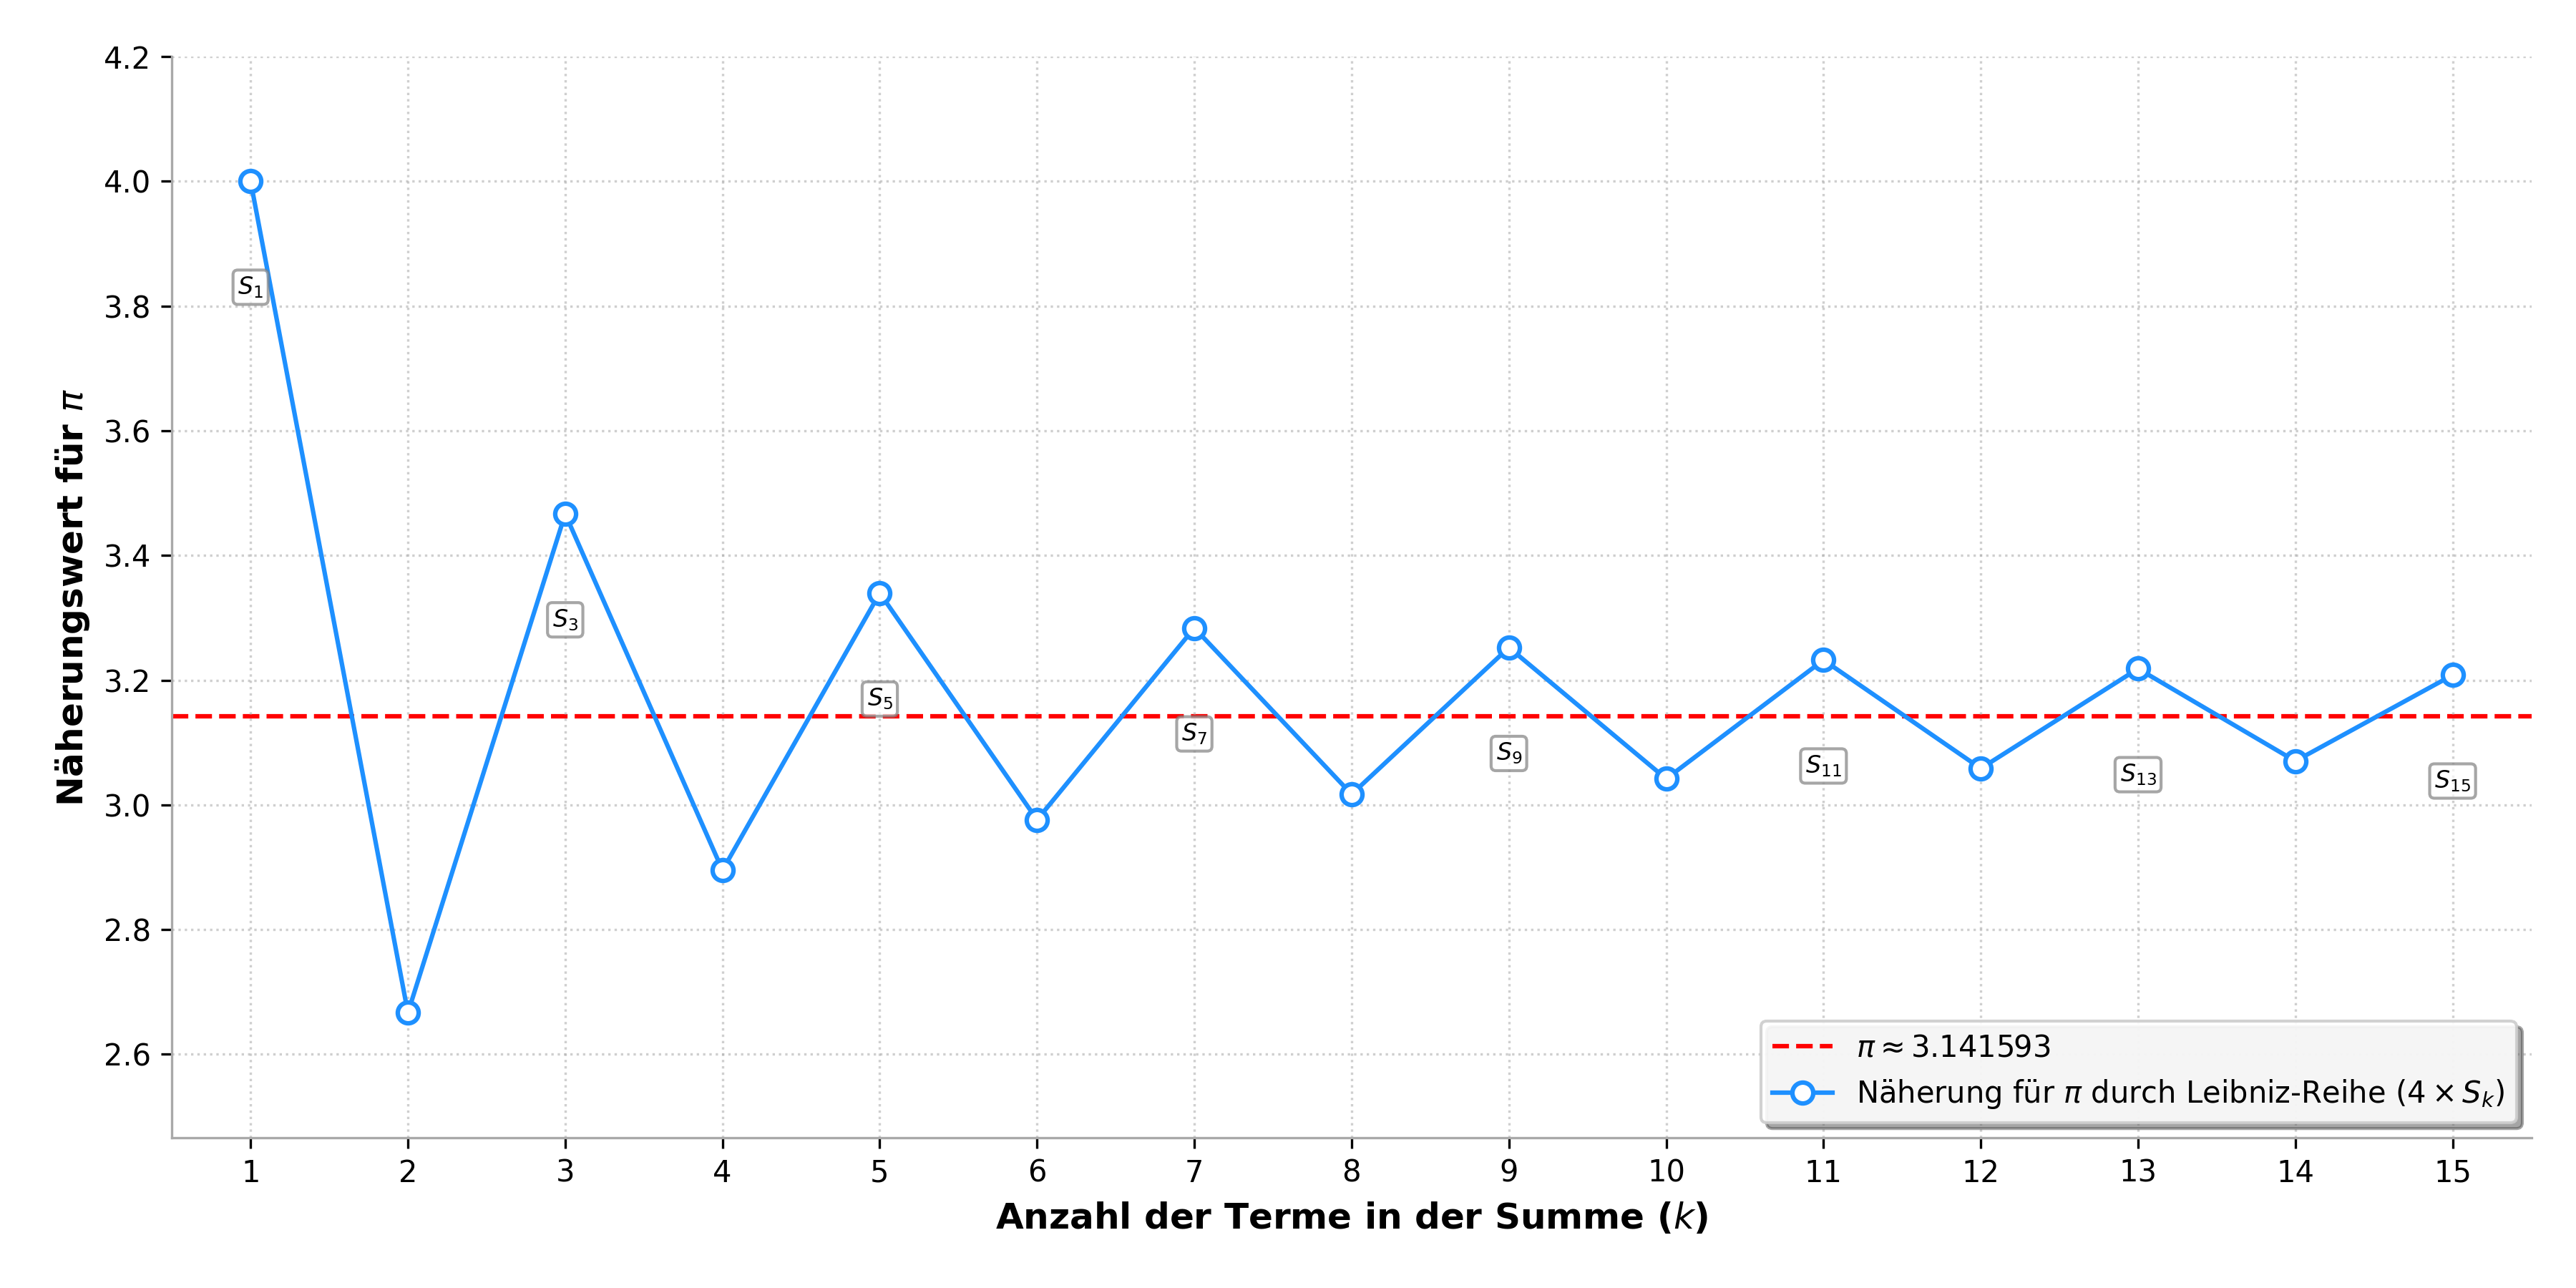
\includegraphics[width=0.8\textwidth]{grafiken/Pi_Leibniz_Reihe.png}
    % Beschreibung für die Grafik 'Pi_Leibniz_Reihe.png':
    % Die Grafik könnte visualisieren, wie sich die Summe der ersten Terme 
    % der Leibniz-Reihe (multipliziert mit 4) langsam dem Wert von Pi annähert.
    % Z.B. ein Zahlenstrahl, auf dem die Näherungswerte für S_1, S_2, S_3 etc. 
    % aufgetragen sind und wie sie um Pi 'oszillieren' und sich annähern.
    % Alternativ: Eine stilisierte Darstellung der Zahl Pi mit der Leibniz-Reihe daneben.
    \captionof{figure}{Annäherung an $\pi$ durch die Leibniz-Reihe (konzeptionelle Darstellung)}
    \label{fig:pi_leibniz_funfact}
\end{center}
\end{funfactbox}

\subsubsection{Ableitungen von Sinus und Kosinus}
Eine der schönsten Symmetrien in der Differentialrechnung findet sich bei den Ableitungen von Sinus und Kosinus.

\begin{infoboxumgebung}{Beobachtung: Steigung von $\sin x$ und Werte von $\cos x$}
Bevor wir die Ableitungsregeln für Sinus und Kosinus formal kennenlernen, lass uns eine kleine Beobachtung am Graphen von $f(x)=\sin(x)$ und $g(x)=\cos(x)$ machen (siehe Abbildung \ref{fig:sincos_graphen}):
\begin{itemize}
    \item Wo hat der Graph von $\sin(x)$ seine Hoch- und Tiefpunkte? Welche Steigung hat der Graph an diesen Stellen offensichtlich? Welchen Wert hat $\cos(x)$ an genau diesen x-Stellen?
    \item Wo schneidet der Graph von $\sin(x)$ die x-Achse mit positiver Steigung (z.B. bei $x=0, 2\pi, \dots$)? Welchen Wert hat $\cos(x)$ dort? Wo ist die Steigung von $\sin(x)$ am größten?
    \item Wo schneidet der Graph von $\sin(x)$ die x-Achse mit negativer Steigung (z.B. bei $x=\pi, 3\pi, \dots$)? Welchen Wert hat $\cos(x)$ dort? Wo ist die Steigung von $\sin(x)$ am stärksten negativ (also betragsmäßig am größten, aber negativ)?
\end{itemize}
Vielleicht erkennst du schon ein Muster im Zusammenhang zwischen der Steigung von $\sin(x)$ und den Funktionswerten von $\cos(x)$. Genau diesen Zusammenhang werden wir mit der Ableitung präzisieren!
\end{infoboxumgebung}

\begin{merksatzumgebung}{Ableitungen von $\sin(x)$ und $\cos(x)$}
Für Winkel $x$ im Bogenmaß gilt:
\begin{itemize}
    \item Die Ableitung von $f(x) = \sin(x)$ ist $f'(x) = \cos(x)$.
    \[ (\sin x)' = \cos x \]
    \item Die Ableitung von $g(x) = \cos(x)$ ist $g'(x) = -\sin(x)$.
    \[ (\cos x)' = -\sin x \]
\end{itemize}
\end{merksatzumgebung}

\begin{tippumgebung}{Ableitungen aus den Taylorreihen (für Interessierte)}
Wenn man die Taylorreihen von $\sin(x)$ und $\cos(x)$ Glied für Glied mit der Potenzregel ableitet (was bei Potenzreihen unter bestimmten Bedingungen erlaubt ist), erhält man genau diese Ableitungsregeln!
Beispiel für Sinus:
$\sin(x) = x - \frac{x^3}{3!} + \frac{x^5}{5!} - \frac{x^7}{7!} + \dots$
$(\sin(x))' = (x)' - (\frac{x^3}{6})' + (\frac{x^5}{120})' - \dots$
$= 1 - \frac{3x^2}{6} + \frac{5x^4}{120} - \dots$
$= 1 - \frac{x^2}{2} + \frac{x^4}{24} - \dots$
$= 1 - \frac{x^2}{2!} + \frac{x^4}{4!} - \dots = \cos(x)$!
\end{tippumgebung}

Mit diesen Ableitungen können wir nun auch die höheren Ableitungen bestimmen:
\begin{itemize}
    \item $f(x) = \sin(x)$
    \item $f'(x) = \cos(x)$
    \item $f''(x) = (\cos x)' = -\sin(x)$
    \item $f'''(x) = (-\sin x)' = -(\cos x) = -\cos(x)$
    \item $f^{(4)}(x) = (-\cos x)' = -(-\sin x) = \sin(x)$
\end{itemize}
Nach der vierten Ableitung wiederholt sich der Zyklus! Das Gleiche gilt für $\cos(x)$.

\subsubsection{Stammfunktionen von Sinus und Kosinus}
Aus den Ableitungsregeln ergeben sich direkt die Stammfunktionen:

\begin{merksatzumgebung}{Stammfunktionen von $\sin(x)$ und $\cos(x)$}
\begin{itemize}
    \item Eine Stammfunktion von $f(x) = \cos(x)$ ist $F(x) = \sin(x)$, denn $(\sin x)' = \cos x$.
    Also: \[\int \cos(x) \,dx = \sin(x) + C \]
    \item Eine Stammfunktion von $g(x) = \sin(x)$ ist $G(x) = -\cos(x)$, denn $(-\cos x)' = -(-\sin x) = \sin x$.
    Also: \[\int \sin(x) \,dx = -\cos(x) + C \]
\end{itemize}
Achte auf das Minuszeichen bei der Stammfunktion von $\sin(x)$!
\end{merksatzumgebung}

\begin{beispielumgebung}{Ableiten und Integrieren mit $\sin x$ und $\cos x$}
\begin{enumerate}
    \item Leite $f(x) = 3\sin(x) - 2\cos(x) + x^2$ ab.
        $f'(x) = (3\sin x)' - (2\cos x)' + (x^2)'$
        $f'(x) = 3\cos(x) - 2(-\sin x) + 2x = 3\cos(x) + 2\sin(x) + 2x$.
    \item Bestimme $\int (4\cos(x) + \sin(x) - 2) \,dx$.
        $\int (4\cos(x) + \sin(x) - 2) \,dx = 4\int\cos(x)dx + \int\sin(x)dx - \int 2dx$
        $= 4\sin(x) + (-\cos x) - 2x + C = 4\sin(x) - \cos(x) - 2x + C$.
\end{enumerate}
\end{beispielumgebung}

\begin{aufgabenumgebung}{Erste Übungen mit $\sin x$ und $\cos x$}
\begin{enumerate}
    \item Bilde die erste und zweite Ableitung der folgenden Funktionen:
        \begin{itemize}
            \item $f_1(x) = -5\cos(x) + 2\sin(x) - e^x$
            \item $f_2(x) = \sin(x) + \ln(x)$ (Beachte den Definitionsbereich!)
        \end{itemize}
    \item Bestimme die Menge aller Stammfunktionen:
        \begin{itemize}
            \item $g_1(x) = \frac{1}{2}\sin(x) - 3\cos(x) + x^3$
            \item $g_2(x) = \cos(x) - \frac{1}{x}$
        \end{itemize}
    \item Berechne das bestimmte Integral $\int_0^{\pi} \sin(x) \,dx$. Was stellt dieser Wert geometrisch dar? Skizziere den Graphen von $\sin(x)$ im Intervall $[0, 2\pi]$ und markiere die berechnete Fläche.
    \item Was ist $\int_0^{2\pi} \sin(x) \,dx$? Erkläre das Ergebnis anhand der Symmetrie und der orientierten Fläche.
\end{enumerate}
\end{aufgabenumgebung}

% Vorheriger Inhalt des Kapitels bis zur aufgabenumgebung 'Erste Übungen mit sin x und cos x'
% ... (siehe vorherige Canvas-Version) ...

% Hier geht es dann weiter mit Transformationen von sin/cos, Tangens, 
% Anwendung der Produkt-/Quotienten-/Kettenregel und Kurvendiskussionen.
% Dieser Kommentar wird durch den folgenden Inhalt ersetzt:

\subsection{Transformationen von Sinus- und Kosinusfunktionen}
\label{subsec:trafo_sincos}

Die Grundfunktionen $f(x)=\sin(x)$ und $g(x)=\cos(x)$ können durch verschiedene Parameter verändert (transformiert) werden, um eine größere Vielfalt an periodischen Vorgängen zu modellieren. Die allgemeine Form einer transformierten Sinusfunktion (analog für Kosinus) ist:
\[ f(x) = A \cdot \sin(B(x-C)) + D \]
oder auch oft geschrieben als:
\[ f(x) = A \cdot \sin(Bx - \varphi) + D \quad \text{mit } \varphi = B \cdot C \]

\begin{merksatzumgebung}{Parameter der allgemeinen Sinusfunktion $f(x) = A \sin(B(x-C)) + D$}
\begin{itemize}
    \item \textbf{Amplitude $|A|$:}
        \begin{itemize}
            \item Der Faktor $A$ streckt oder staucht den Graphen in y-Richtung.
            \item $|A|$ ist die \textbf{Amplitude}, d.h. die maximale Auslenkung von der Mittellage. Der Wertebereich ist $[D-|A|, D+|A|]$.
            \item Wenn $A < 0$, wird der Graph zusätzlich an der Mittellage (Gerade $y=D$) gespiegelt.
        \end{itemize}
    \item \textbf{Periode $P$ (beeinflusst durch $B$):}
        \begin{itemize}
            \item Der Faktor $B$ beeinflusst die Periode der Schwingung. $B$ wird auch Kreisfrequenz genannt (oft als $\omega$ bezeichnet).
            \item Die \textbf{Periode} $P$ (die Länge einer vollständigen Schwingung) berechnet sich als:
            \[ P = \frac{2\pi}{|B|} \]
            \item Wenn $|B|>1$, wird die Periode kürzer (die Schwingung ist 'schneller', gestaucht in x-Richtung).
            \item Wenn $0<|B|<1$, wird die Periode länger (die Schwingung ist 'langsamer', gestreckt in x-Richtung).
            \item \textit{Zum Weiterdenken:} Was passiert anschaulich mit der Periode $P$, wenn der Betrag von $B$ sehr groß wird (z.B. $|B|=100$)? Die Schwingung wird dann sehr \dots (schnell/kurz oder langsam/lang)? Und was passiert, wenn $|B|$ sehr klein (aber positiv) wird (z.B. $|B|=0.1$)? Die Schwingung wird dann sehr \dots? Passt das zu deiner Vorstellung von 'gestaucht' bzw. 'gestreckt' in x-Richtung?
        \end{itemize}
    \item \textbf{Verschiebung in x-Richtung (Phasenverschiebung $C$):}
        \begin{itemize}
            \item Der Parameter $C$ bewirkt eine Verschiebung des Graphen entlang der x-Achse.
            \item Wenn $C>0$ (also im Term $(x-C)$), wird der Graph um $C$ Einheiten nach \textbf{rechts} verschoben.
            \item Wenn $C<0$ (also im Term $(x+ |C|)$), wird der Graph um $|C|$ Einheiten nach \textbf{links} verschoben.
            \item Diese Verschiebung wird auch \textbf{Phasenverschiebung} genannt.
        \end{itemize}
    \item \textbf{Verschiebung in y-Richtung (Mittellage $D$):}
        \begin{itemize}
            \item Der Parameter $D$ verschiebt den gesamten Graphen um $D$ Einheiten in y-Richtung.
            \item Die Gerade $y=D$ ist die neue \textbf{Mittellage} oder Ruhelage der Schwingung.
        \end{itemize}
\end{itemize}
Die gleichen Interpretationen gelten für die Kosinusfunktion $f(x) = A \cos(B(x-C)) + D$.
\end{merksatzumgebung}

\begin{beispielumgebung}{Analyse einer transformierten Sinusfunktion}
Betrachte die Funktion $f(x) = 2 \sin\left(0.5(x - \frac{\pi}{2})\right) + 1$.
\begin{itemize}
    \item \textbf{Amplitude $A$:} $A=2$. Die maximale Auslenkung von der Mittellage ist 2.
    \item \textbf{Parameter $B$ und Periode $P$:} $B=0.5$. Die Periode ist $P = \frac{2\pi}{|0.5|} = \frac{2\pi}{1/2} = 4\pi$. Die Schwingung ist also langsamer als die Grundschwingung.
    \item \textbf{Verschiebung in x-Richtung $C$:} $C=\frac{\pi}{2}$. Der Graph der Sinusfunktion $2\sin(0.5x)$ wird um $\frac{\pi}{2}$ nach rechts verschoben.
    \item \textbf{Verschiebung in y-Richtung $D$:} $D=1$. Die Mittellage ist die Gerade $y=1$.
    \item \textbf{Wertebereich:} Die Mittellage ist $y=1$, die Amplitude ist $2$. Also schwingt die Funktion zwischen $1-2=-1$ und $1+2=3$. Der Wertebereich ist $[-1, 3]$.
\end{itemize}
\begin{center}
    % Platzhalter für die Grafik 'Transformierte Sinusfunktion'
    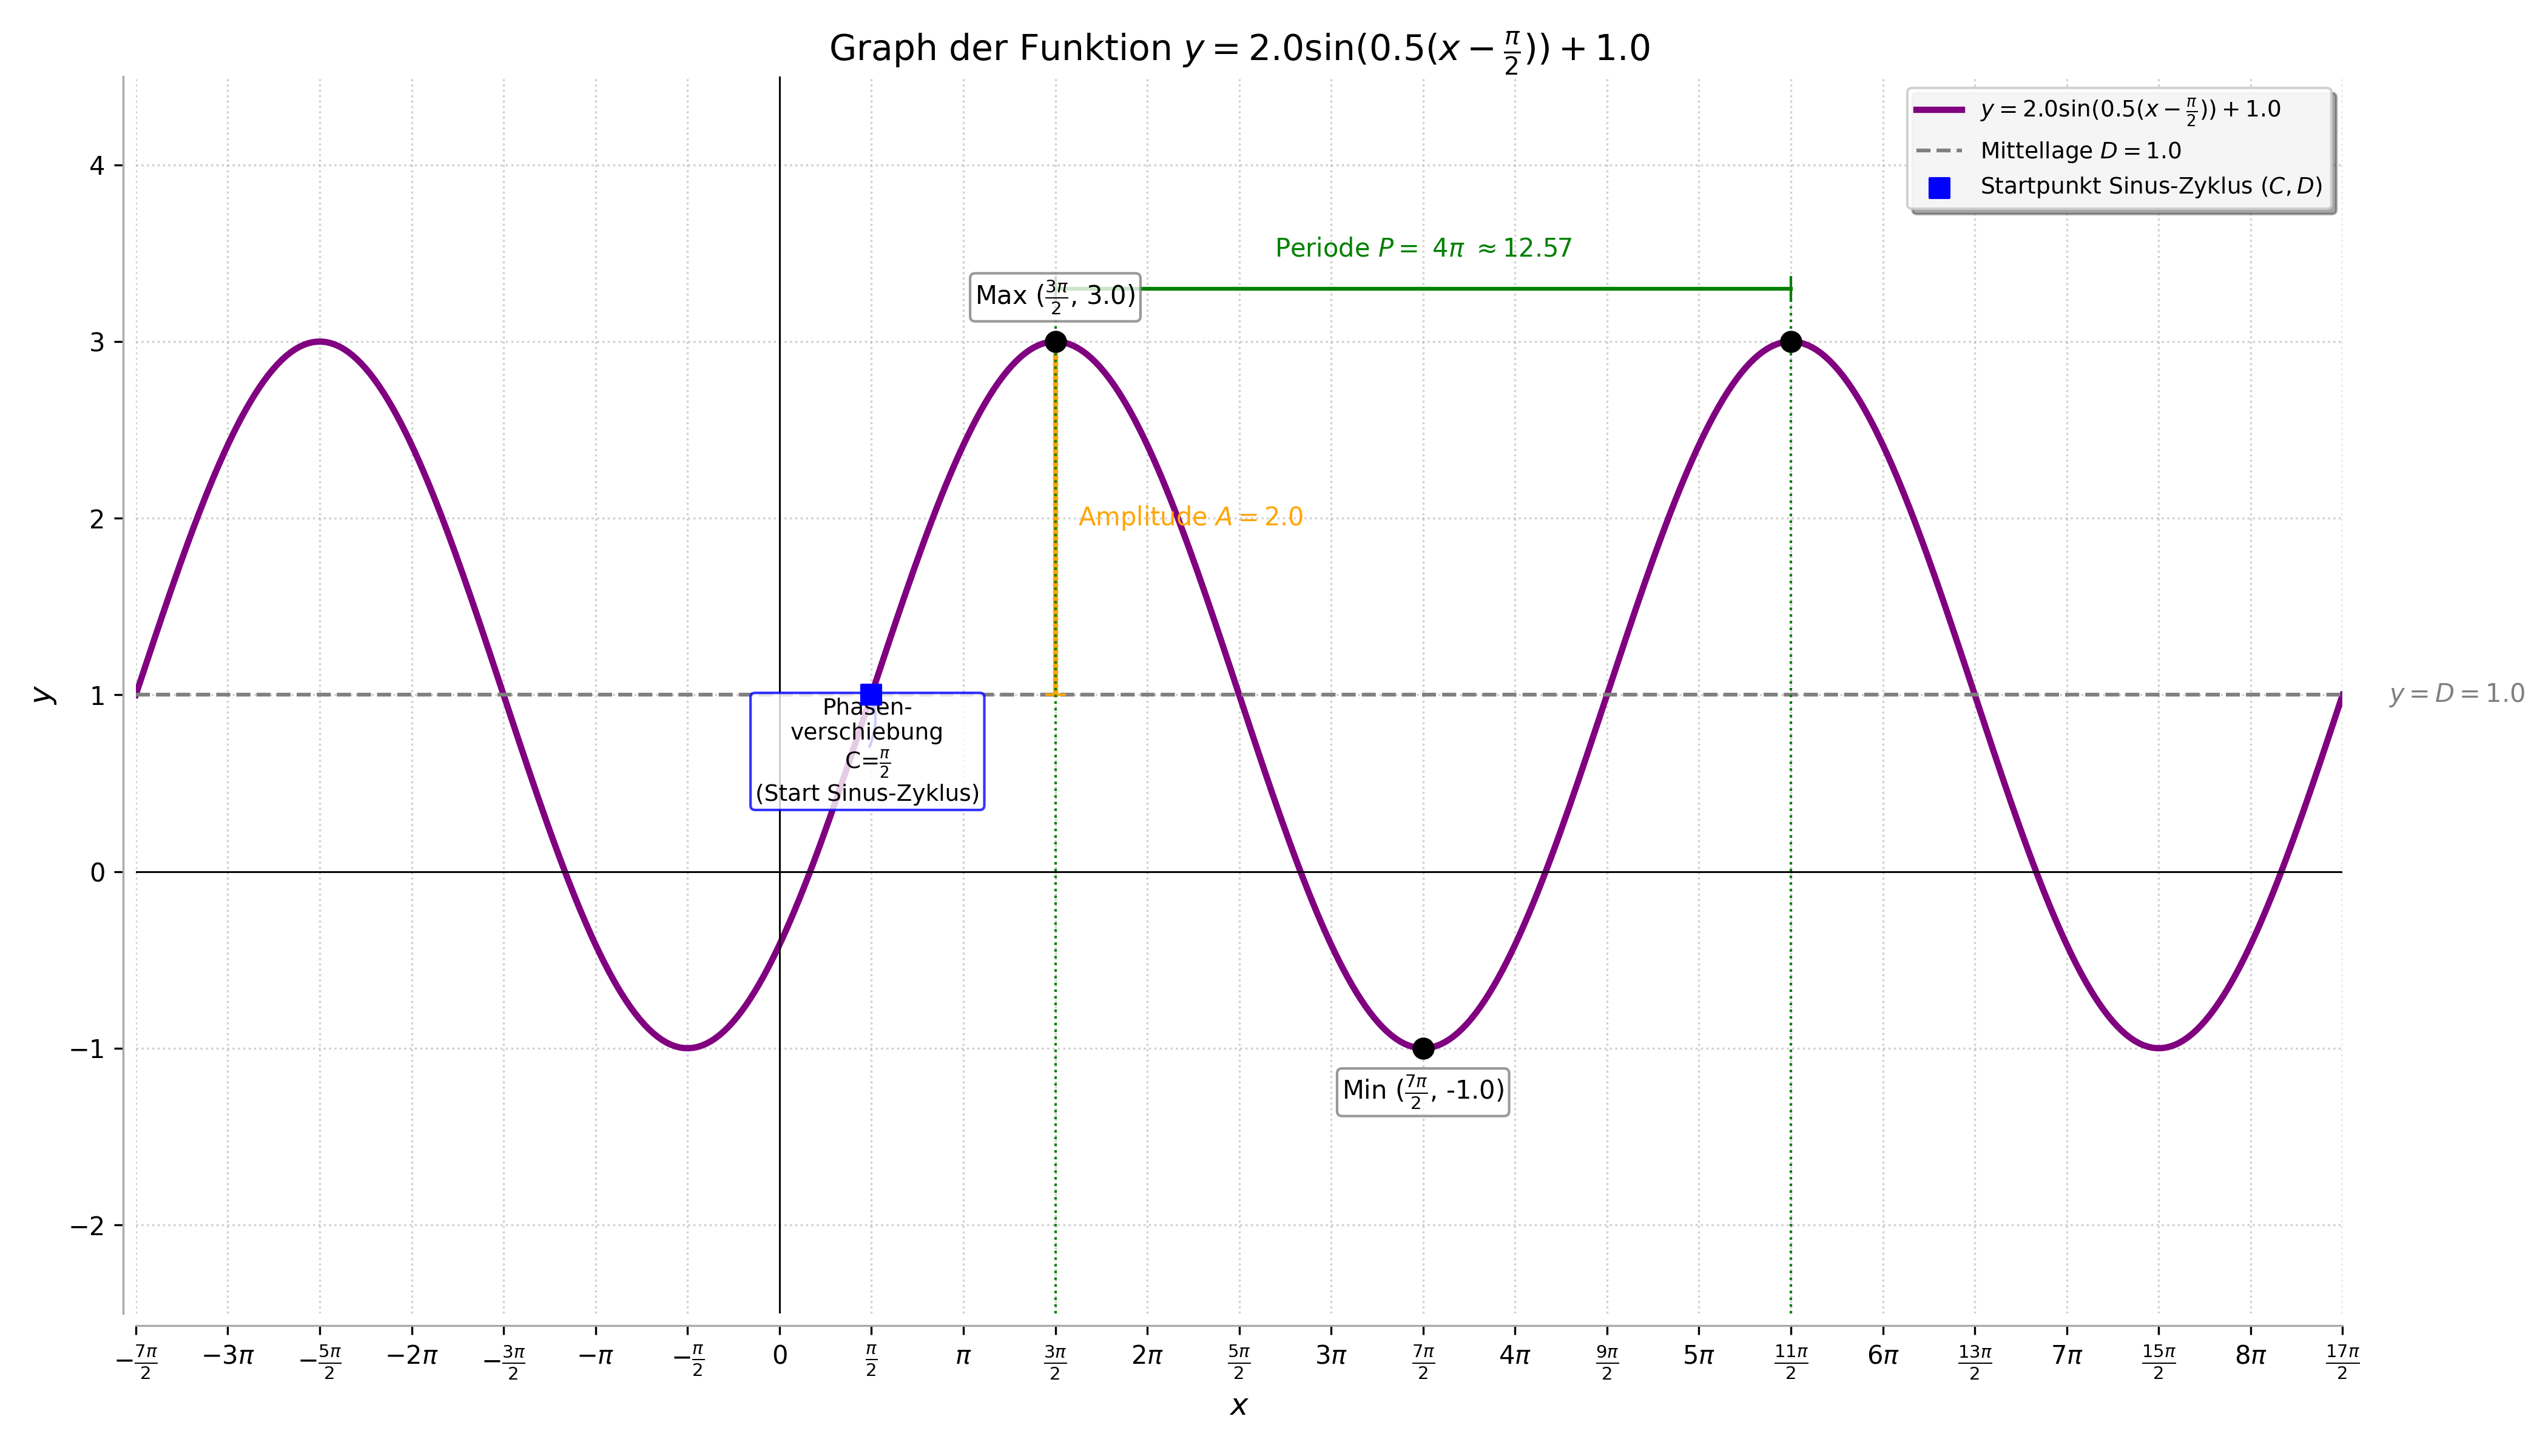
\includegraphics[width=0.9\textwidth]{grafiken/Trig_Trafo_Sinus.png}
    \captionof{figure}{Graph der transformierten Sinusfunktion.}
    \label{fig:trafo_sin}
\end{center}
\end{beispielumgebung}

\begin{fehlerboxumgebung}{Trigonometrische Funktionen – Typische Fallstricke}
Beim Rechnen mit Sinus, Kosinus und Co. gibt es einige typische Fehlerquellen:
\begin{itemize}
    \item \textbf{Gradmaß vs. Bogenmaß:} Die Ableitungs- und Integrationsregeln $(\sin x)'=\cos x$ etc. gelten \textbf{nur}, wenn $x$ im Bogenmaß angegeben ist! Viele Taschenrechner sind standardmäßig auf Gradmaß (DEG) eingestellt. Für die Analysis muss er auf Radiant (RAD) umgestellt sein, sonst sind numerische Ergebnisse falsch.
    \item \textbf{Vorzeichen bei Ableitungen/Stammfunktionen:} Merke dir gut: $(\cos x)' = \mathbf{-}\sin x$ und $\int \sin x \,dx = \mathbf{-}\cos x + C$. Diese Minuszeichen werden oft vergessen!
    \item \textbf{Parameter bei Transformationen falsch interpretiert:}
        \begin{itemize}
            \item Bei $A \sin(B(x-C))+D$: Die Periode ist $P=\frac{2\pi}{|B|}$, nicht $2\pi \cdot B$ oder Ähnliches.
            \item Die Phasenverschiebung bei $B(x-C)$ ist $C$ nach rechts. Steht z.B. $\sin(2x-\pi)$, musst du erst $2$ ausklammern zu $\sin(2(x-\frac{\pi}{2}))$, um die korrekte Phasenverschiebung $C=\frac{\pi}{2}$ nach rechts zu erkennen.
        \end{itemize}
    \item \textbf{Definitionsbereich von $\tan x$ ignoriert:} $\tan x$ ist nicht für $x = \frac{\pi}{2} + k\pi$ definiert. An diesen Stellen sind Polstellen (senkrechte Asymptoten).
    \item \textbf{Verwechslung von $\sin^2 x$ mit $\sin(x^2)$:} $\sin^2 x = (\sin x)^2$, während $\sin(x^2)$ bedeutet, dass zuerst $x$ quadriert und dann der Sinus davon genommen wird. Beim Ableiten erfordern sie unterschiedliche Anwendungen der Kettenregel.
\end{itemize}
Achte auf diese Punkte, um typische Fehler zu vermeiden!
\end{fehlerboxumgebung}

\begin{aufgabenumgebung}{Transformierte Sinus- und Kosinusfunktionen}
\begin{enumerate}
    \item Bestimme für die folgenden Funktionen Amplitude, Periode, Phasenverschiebung (Richtung und Betrag) und Verschiebung in y-Richtung. Gib den Wertebereich an.
        \begin{itemize}
            \item $f_1(x) = 3 \cos(2x - \pi) - 1$ (Tipp: Klammere zuerst den Faktor vor dem $x$ in der Klammer aus, um die Form $B(x-C)$ zu erhalten: $2x-\pi = 2(x-\frac{\pi}{2})$)
            \item $f_2(x) = -0.5 \sin(\pi x + \frac{\pi}{4}) + 2$
            \item $f_3(t) = 100 \cos(2\pi \cdot 50 t)$ (Modell für Wechselspannung)
        \end{itemize}
    \item Skizziere den Graphen von $g(x) = \sin(2(x+\frac{\pi}{4}))$ für eine Periode. Beginne mit dem Graphen von $\sin(x)$ und führe die Transformationen schrittweise durch.
    \item Gegeben ist ein Graph einer Sinusfunktion. Bestimme aus dem Graphen die Parameter $A, B, C, D$ und stelle eine mögliche Funktionsgleichung auf.
        \begin{center}
            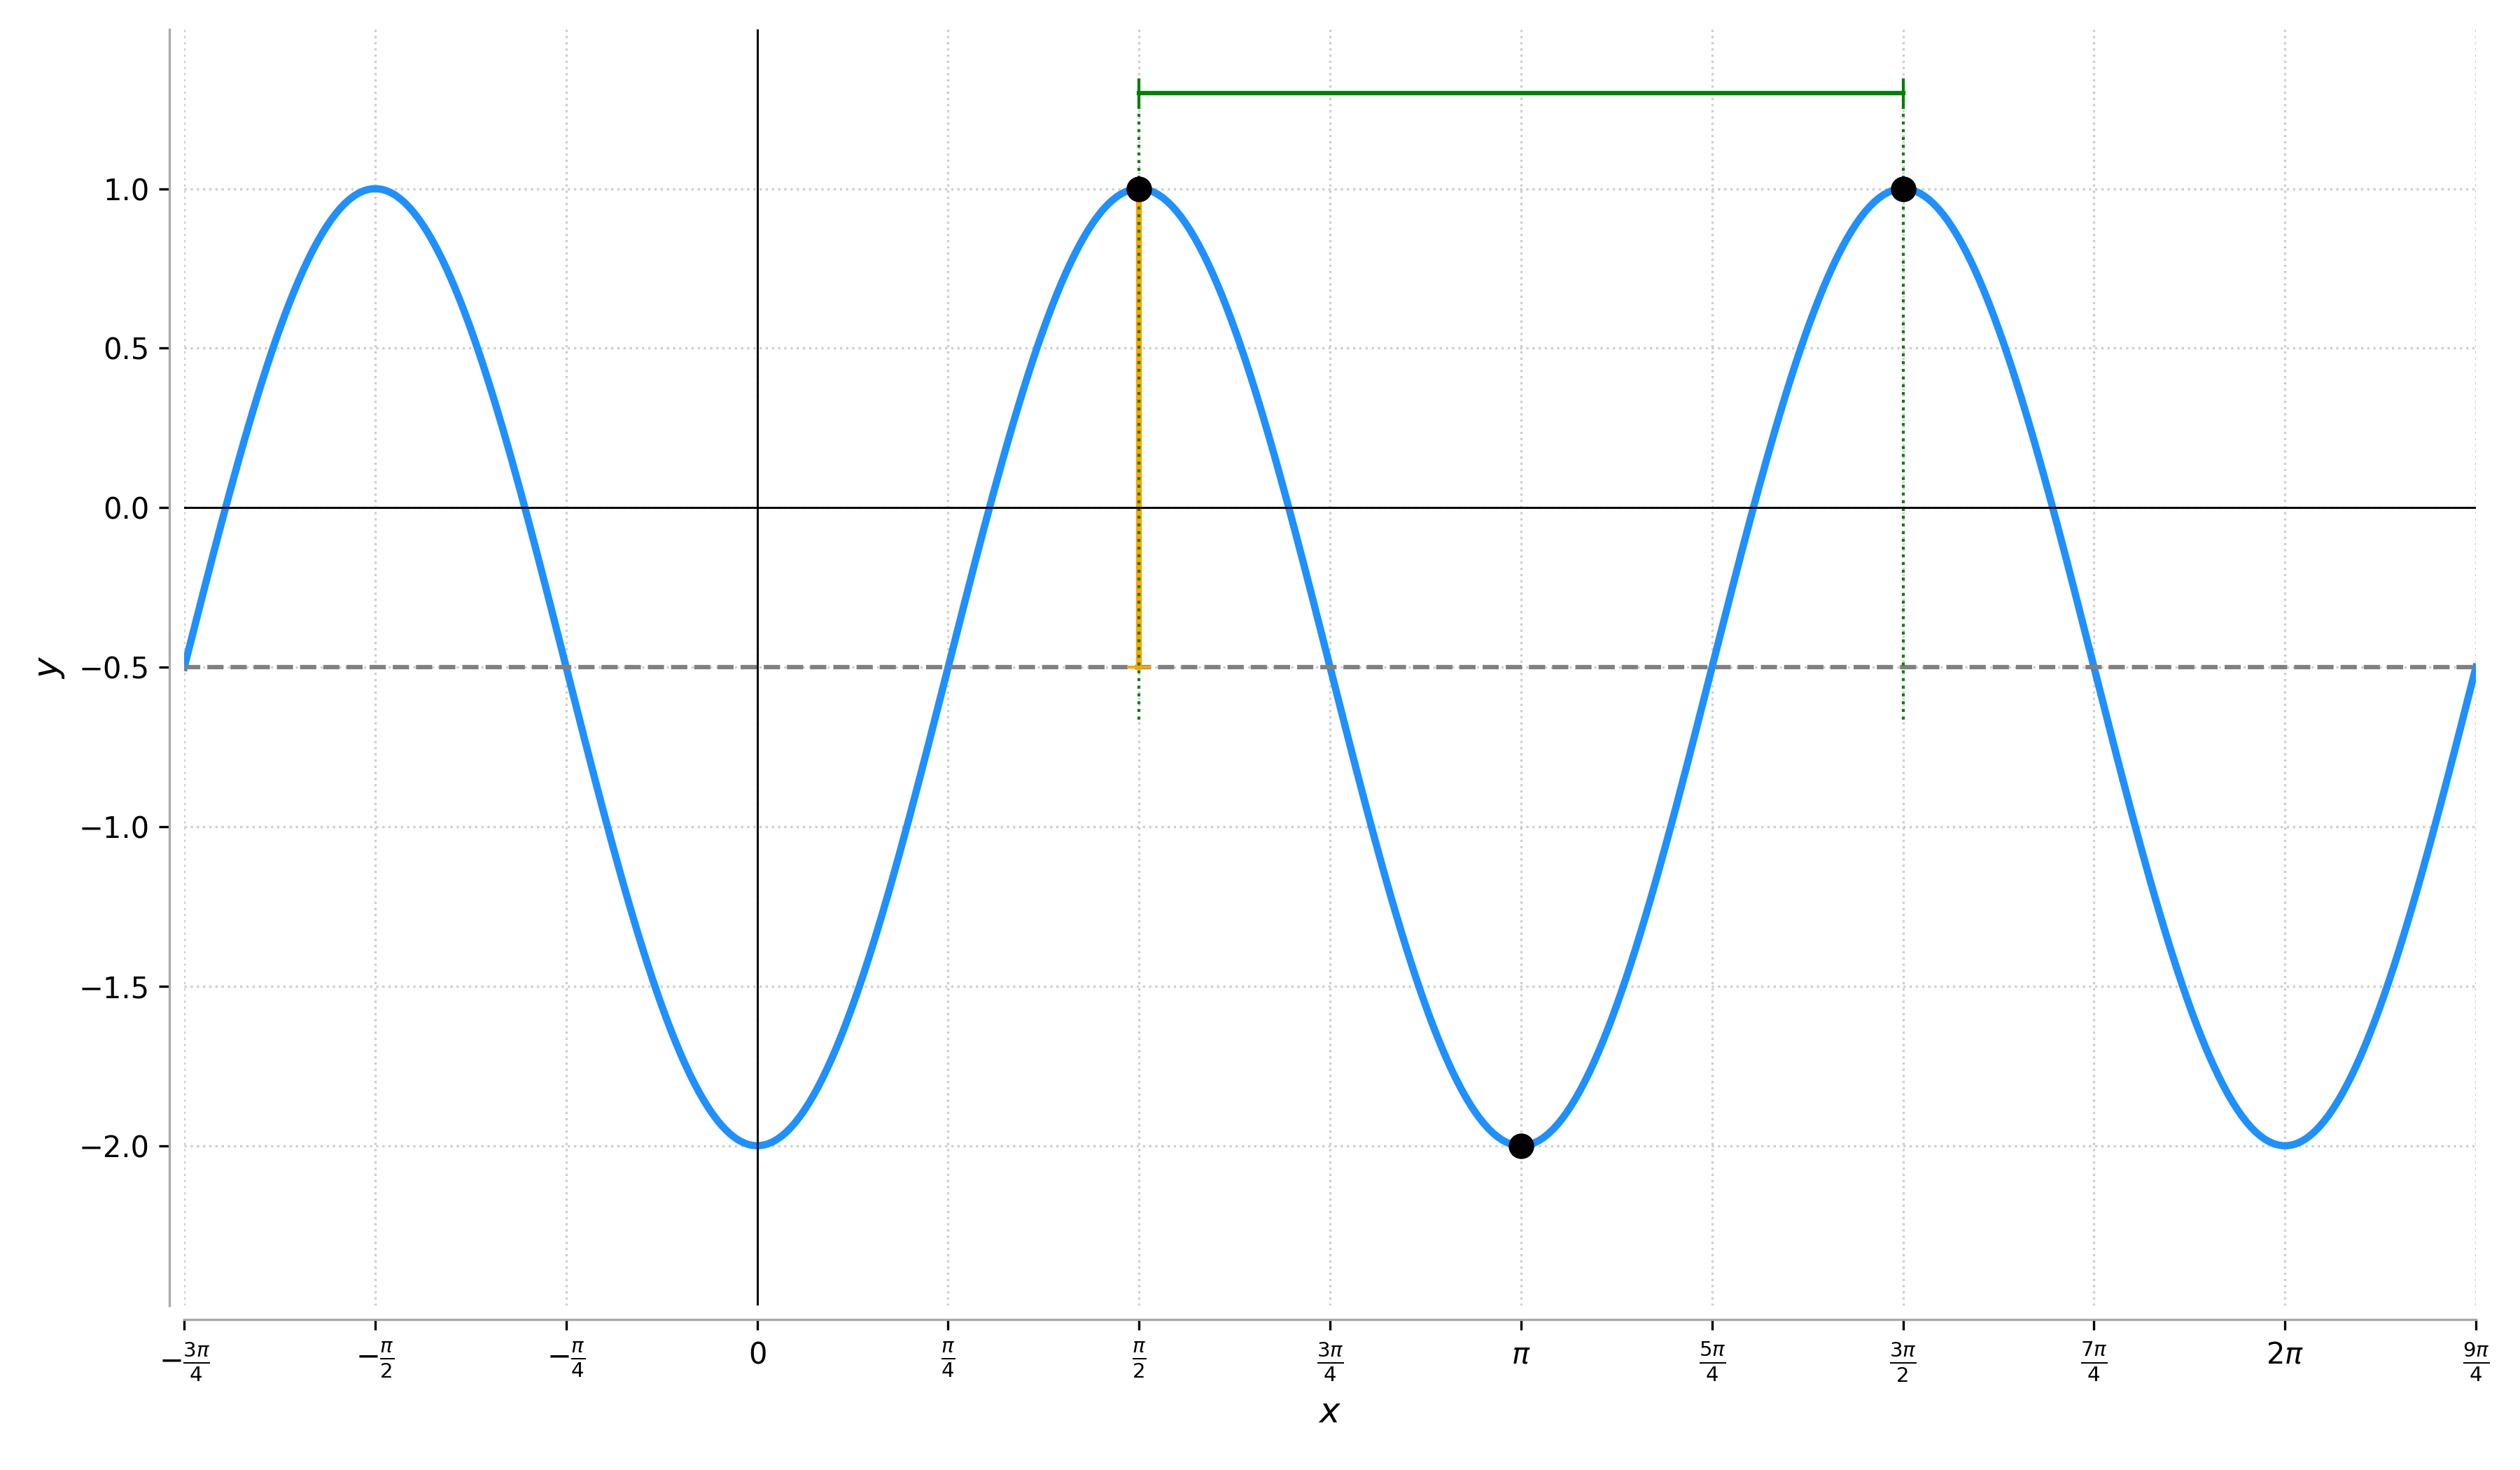
\includegraphics[width=0.7\textwidth]{grafiken/Trig_Graph_Ablesen.png}
            \captionof{figure}{Graph zum Ablesen der Parameter}
            \label{fig:graph_ablesen}
        \end{center}
\end{enumerate}
\end{aufgabenumgebung}

\subsection{Die Tangensfunktion ($\tan x$) und Kotangensfunktion ($\cot x$)}
\label{subsec:tangens_kotangens}

Neben Sinus und Kosinus gibt es weitere wichtige trigonometrische Funktionen. Die bekannteste davon ist die Tangensfunktion.

\begin{merksatzumgebung}{Definition der Tangensfunktion ($\tan x$)}
Die \textbf{Tangensfunktion} ist definiert als das Verhältnis von Sinus zu Kosinus:
\[ \tan(x) = \frac{\sin(x)}{\cos(x)} \]
\textbf{Geometrische Deutung am Einheitskreis:}
Die Tangensfunktion entspricht der y-Koordinate des Punktes, an dem der verlängerte freie Schenkel des Winkels $x$ die Tangente an den Einheitskreis im Punkt $(1|0)$ schneidet. Sie kann auch als Steigung des freien Schenkels des Winkels $x$ interpretiert werden.

\textbf{Eigenschaften von $f(x)=\tan(x)$:}
\begin{itemize}
    \item \textbf{Definitionsbereich:} $D_f = \mathbb{R} \setminus \{ \frac{\pi}{2} + k\pi \,|\, k \in \mathbb{Z} \}$.
    Der Tangens ist nicht definiert, wenn $\cos(x)=0$ ist (also an den Nullstellen des Kosinus), da man nicht durch Null teilen darf. An diesen Stellen hat der Graph \textbf{senkrechte Asymptoten}.
    \item \textbf{Wertebereich:} $W_f = \mathbb{R}$ (der Tangens kann jeden reellen Wert annehmen).
    \item \textbf{Periodizität:} Die Tangensfunktion ist periodisch mit der \textbf{Periode $\pi$}.
        \[ \tan(x + \pi) = \tan(x) \]
        (Beachte: kürzere Periode als Sinus und Kosinus!)
    \item \textbf{Nullstellen:} $\tan(x) = 0 \Leftrightarrow \sin(x)=0$. Also für $x = k \cdot \pi$, wobei $k \in \mathbb{Z}$.
    \item \textbf{Symmetrie:} $\tan(x)$ ist \textbf{punktsymmetrisch zum Ursprung}: $\tan(-x) = \frac{\sin(-x)}{\cos(-x)} = \frac{-\sin x}{\cos x} = -\tan(x)$.
    \item \textbf{Monotonie:} Die Tangensfunktion ist in jedem ihrer Definitionsintervalle streng monoton steigend.
\end{itemize}
\end{merksatzumgebung}

\begin{center}
    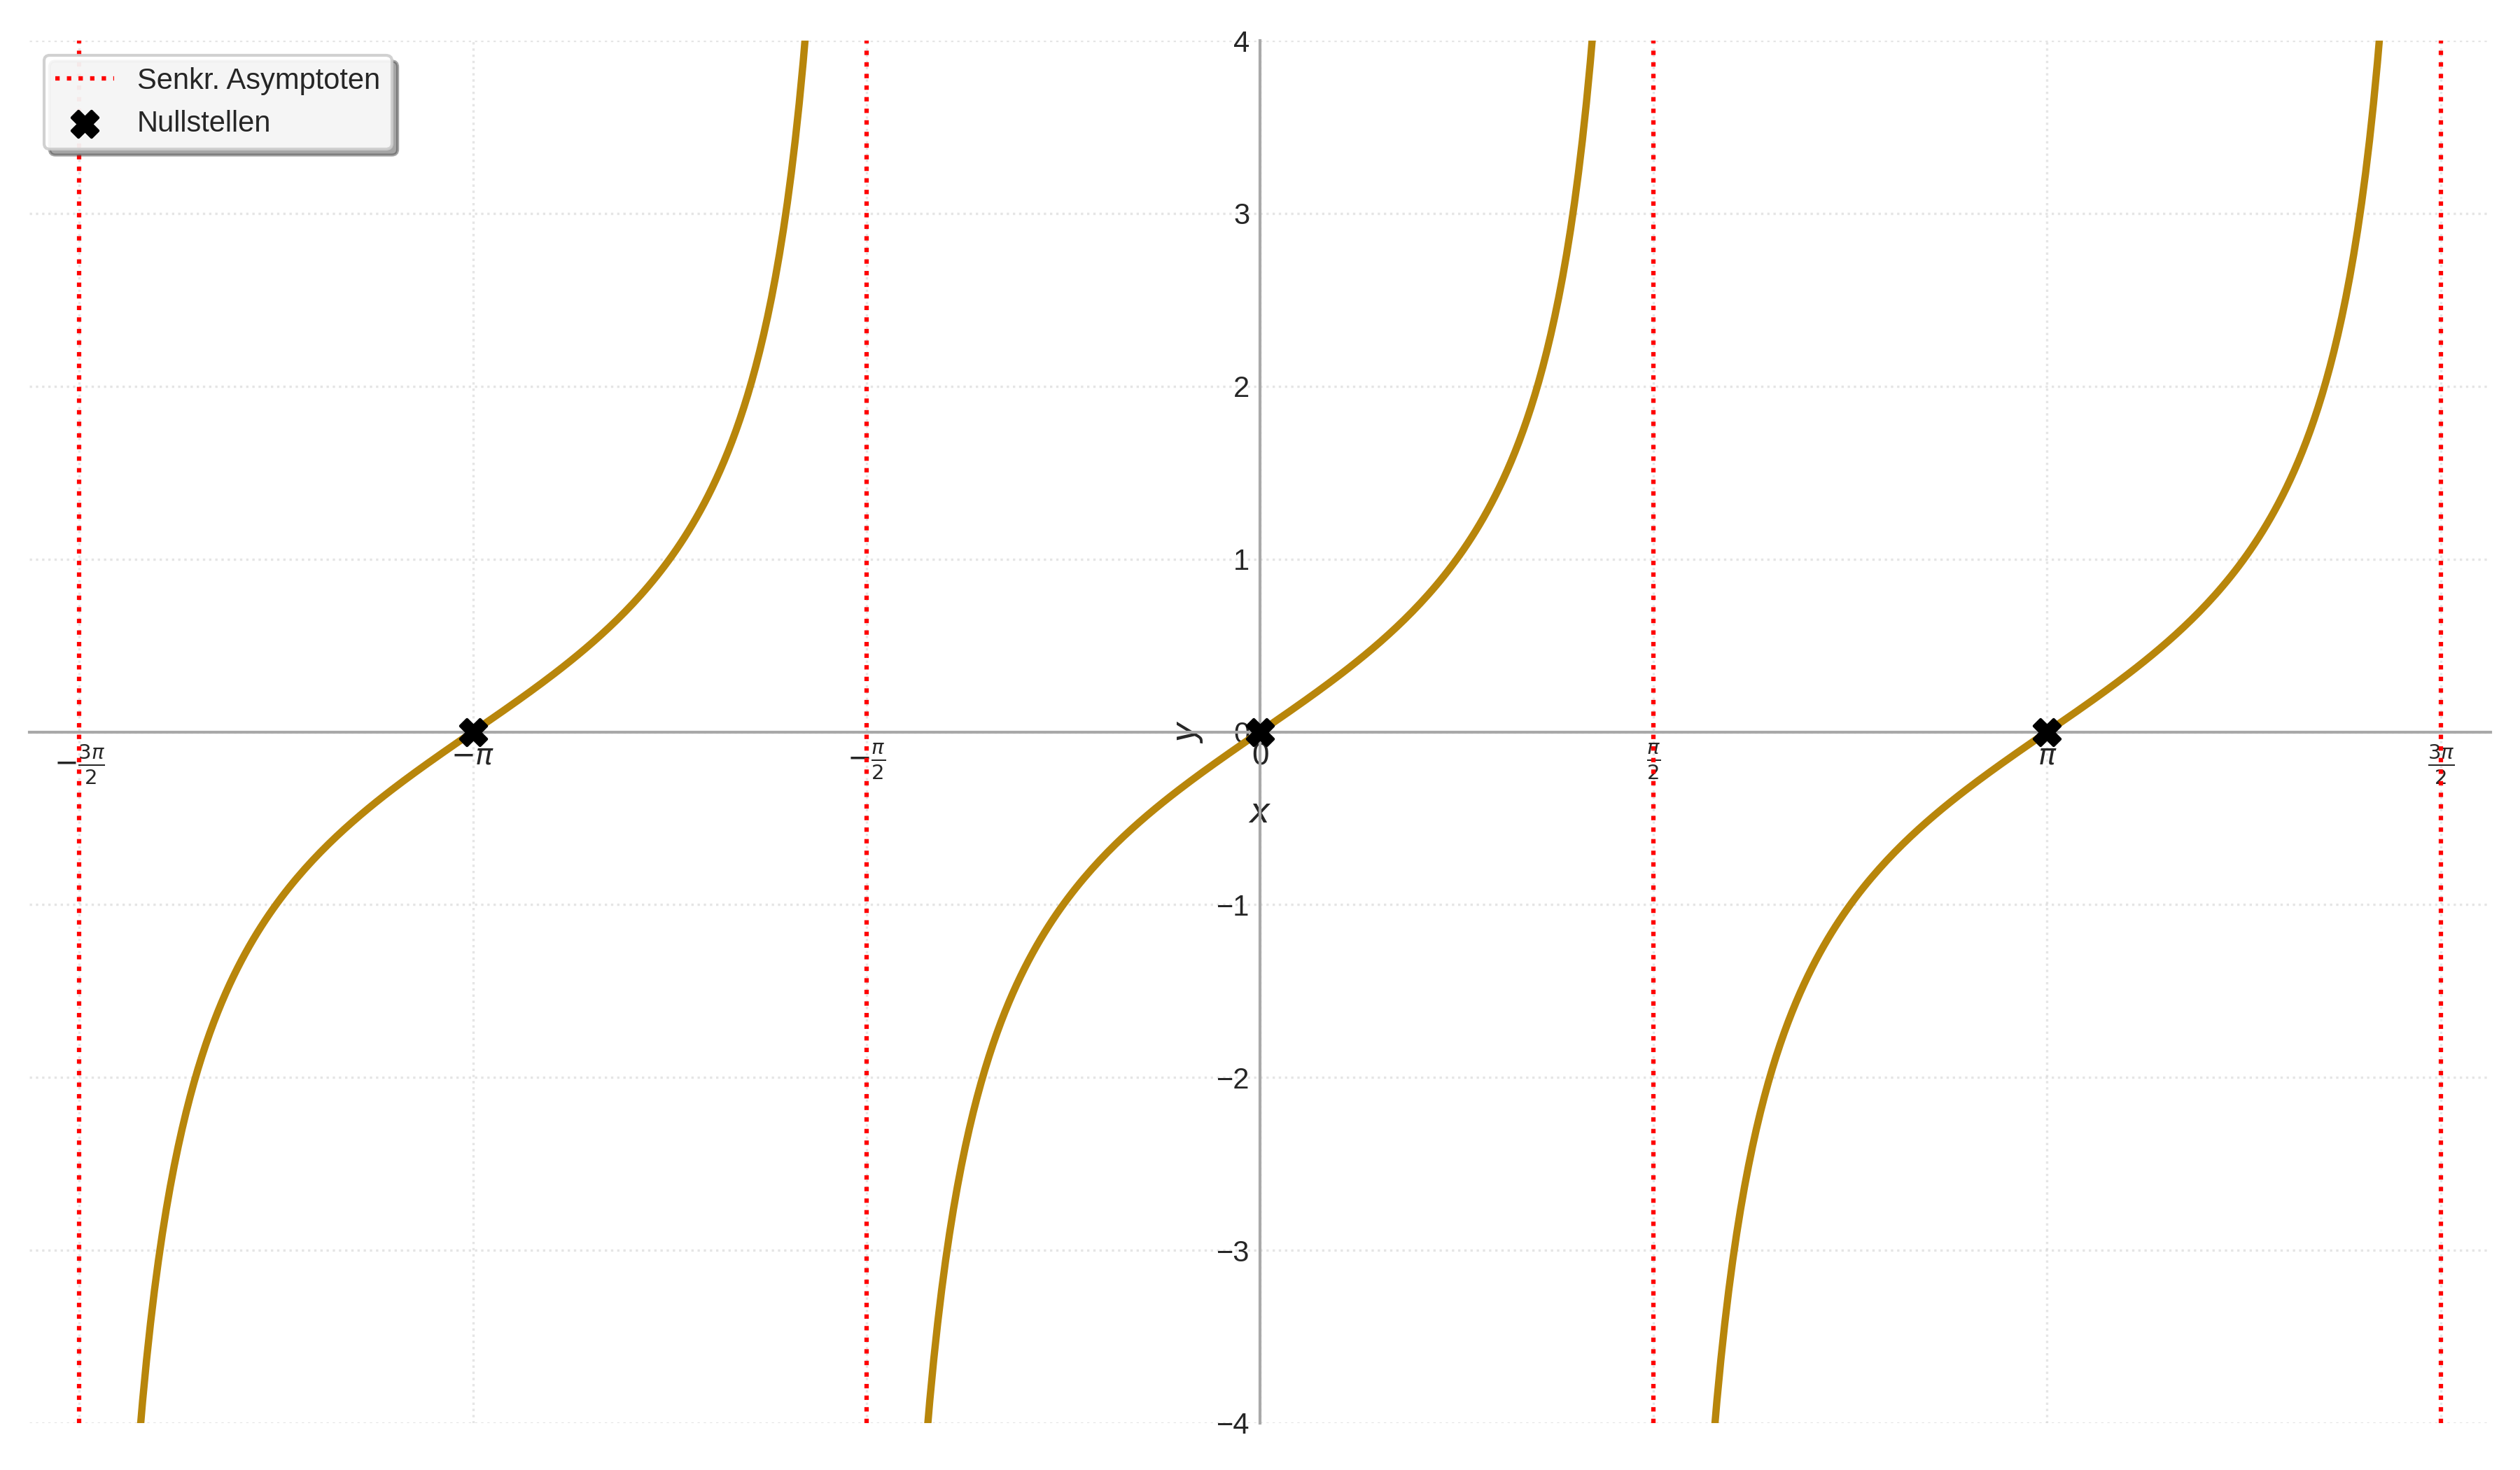
\includegraphics[width=0.9\textwidth]{grafiken/Trig_Tangens_Graph.png}
    \captionof{figure}{Graph der Funktion $f(x)=\tan(x)$}
    \label{fig:tangens_graph}
\end{center}

\begin{infoboxumgebung}{Die Kotangensfunktion ($\cot x$)}
Die \textbf{Kotangensfunktion} ist definiert als $\cot(x) = \frac{\cos(x)}{\sin(x)} = \frac{1}{\tan(x)}$.
Sie ist nicht definiert, wenn $\sin(x)=0$ ist (also bei $x=k\pi$). Ihre Periode ist ebenfalls $\pi$.
Der Kotangens spielt in der Schulmathematik oft eine geringere Rolle als der Tangens, ist aber in manchen Anwendungen nützlich.
\end{infoboxumgebung}

\subsubsection{Ableitungen von Tangens (und Kotangens)}
Die Ableitung der Tangensfunktion können wir mit der Quotientenregel herleiten.

\begin{merksatzumgebung}{Ableitung von $\tan(x)$ und $\cot(x)$}
\begin{itemize}
    \item Die Ableitung von $f(x) = \tan(x)$ ist:
    \[ (\tan x)' = \frac{1}{\cos^2(x)} = 1 + \tan^2(x) \]
    \item Die Ableitung von $g(x) = \cot(x)$ ist:
    \[ (\cot x)' = -\frac{1}{\sin^2(x)} = -(1 + \cot^2(x)) \]
\end{itemize}
\end{merksatzumgebung}

\textbf{Herleitung der Ableitung von $\tan(x)$:}
Wir verwenden $\tan(x) = \frac{\sin(x)}{\cos(x)}$ und die Quotientenregel $(\frac{u}{v})' = \frac{u'v - uv'}{v^2}$.
Sei $u(x) = \sin(x) \implies u'(x) = \cos(x)$.
Sei $v(x) = \cos(x) \implies v'(x) = -\sin(x)$.
$(\tan x)' = \frac{(\cos x)(\cos x) - (\sin x)(-\sin x)}{(\cos x)^2} = \frac{\cos^2(x) + \sin^2(x)}{\cos^2(x)}$.
Mit dem trigonometrischen Pythagoras $\sin^2(x) + \cos^2(x) = 1$ folgt:
$(\tan x)' = \frac{1}{\cos^2(x)}$.
Alternative Form: $\frac{1}{\cos^2(x)} = \frac{\cos^2(x) + \sin^2(x)}{\cos^2(x)} = \frac{\cos^2(x)}{\cos^2(x)} + \frac{\sin^2(x)}{\cos^2(x)} = 1 + \left(\frac{\sin x}{\cos x}\right)^2 = 1 + \tan^2(x)$.

\begin{aufgabenumgebung}{Ableiten mit Tangens}
Bilde die erste Ableitung der folgenden Funktionen:
\begin{enumerate}
    \item $f(x) = 3\tan(x) - x$
    \item $g(x) = x \cdot \tan(x)$ (Produktregel!)
    \item $h(x) = \tan(2x+1)$ (Kettenregel! Äußere Funktion $\tan(u)$, innere $u=2x+1$)
\end{enumerate}
\end{aufgabenumgebung}

\subsection{Anwendung der Ableitungsregeln auf trigonometrische Funktionen}
\label{subsec:ableitungsregeln_trig}

Jetzt kombinieren wir Sinus, Kosinus (und Tangens) mit Polynomen oder anderen Funktionen und wenden unsere bekannten Ableitungsregeln (Produkt-, Quotienten-, Kettenregel) an.

\begin{beispielumgebung}{Kombinierte Ableitungsregeln mit trigonometrischen Funktionen}
\begin{enumerate}
    \item \textbf{Produktregel:} $f(x) = x^2 \sin(x)$.
        $u(x)=x^2 \implies u'(x)=2x$.
        $v(x)=\sin(x) \implies v'(x)=\cos(x)$.
        $f'(x) = u'v + uv' = 2x \sin(x) + x^2 \cos(x)$.

    \item \textbf{Quotientenregel:} $g(x) = \frac{\cos(x)}{x}$. (Für $x \neq 0$)
        $u(x)=\cos(x) \implies u'(x)=-\sin(x)$.
        $v(x)=x \implies v'(x)=1$.
        $g'(x) = \frac{u'v - uv'}{v^2} = \frac{-\sin(x) \cdot x - \cos(x) \cdot 1}{x^2} = \frac{-x\sin(x) - \cos(x)}{x^2}$.

    \item \textbf{Kettenregel:} $h(x) = \sin(3x^2+2)$.
        Äußere Funktion: $a(u)=\sin(u) \implies a'(u)=\cos(u)$.
        Innere Funktion: $b(x)=3x^2+2 \implies b'(x)=6x$.
        $h'(x) = a'(b(x)) \cdot b'(x) = \cos(3x^2+2) \cdot 6x = 6x \cos(3x^2+2)$.

    \item \textbf{Kombination:} $k(x) = e^x \cos(2x)$. (Produkt- und Kettenregel)
        $u(x)=e^x \implies u'(x)=e^x$.
        $v(x)=\cos(2x)$. Für $v'(x)$ brauchen wir die Kettenregel:
            Äußere: $\cos(u) \implies -\sin(u)$. Innere: $2x \implies 2$. Also $v'(x) = -\sin(2x) \cdot 2 = -2\sin(2x)$.
        $k'(x) = u'v + uv' = e^x \cos(2x) + e^x (-2\sin(2x)) = e^x(\cos(2x) - 2\sin(2x))$.
\end{enumerate}
\end{beispielumgebung}

\begin{aufgabenumgebung}{Ableiten trigonometrischer Funktionskombinationen}
Bilde die erste Ableitung der folgenden Funktionen und vereinfache, wenn möglich.
\begin{enumerate}
    \item $f_1(x) = (x^3+1)\cos(x)$
    \item $f_2(x) = \frac{\sin(x)}{e^x}$
    \item $f_3(x) = \cos(x^2+1)$
    \item $f_4(x) = \sin^2(x)$ (Tipp: $\sin^2(x) = (\sin x)^2$. Kettenregel!)
    \item $f_5(x) = \ln(\cos x)$ (Für welche $x$ ist dies definiert?)
    \item $f_6(x) = e^{\sin(x)}$
\end{enumerate}
\end{aufgabenumgebung}

\subsection{Kurvendiskussion von trigonometrischen Funktionen (Beispiele)}
\label{subsec:kurvendiskussion_trig}

Die Kurvendiskussion von reinen Sinus- oder Kosinusfunktionen ist oft einfach, da ihre Eigenschaften (Periode, Amplitude, Nullstellen, Extrema) bekannt sind. Interessanter wird es, wenn sie mit anderen Funktionen kombiniert werden oder transformiert sind.

\begin{beispielumgebung}{Kurvendiskussion von $f(x) = \sin(x) + \cos(x)$ im Intervall $[0, 2\pi]$}
\begin{enumerate}
    \item \textbf{Definitionsbereich:} $D_f = \mathbb{R}$, hier betrachten wir $[0, 2\pi]$.
    \item \textbf{Symmetrie:} $f(-x) = \sin(-x)+\cos(-x) = -\sin(x)+\cos(x)$. Weder achsen- noch punktsymmetrisch zum Ursprung.
    \item \textbf{Grenzwerte:} Nicht relevant für ein abgeschlossenes Intervall. Periodisch mit $P=2\pi$.
    \item \textbf{y-Achsenabschnitt:} $f(0) = \sin(0)+\cos(0) = 0+1=1$. $P_y(0|1)$.
    \item \textbf{Nullstellen:} $f(x)=0 \implies \sin(x)+\cos(x)=0 \implies \sin(x)=-\cos(x)$.
        Wenn $\cos(x) \neq 0$, können wir teilen: $\frac{\sin x}{\cos x} = -1 \implies \tan(x)=-1$.
        Im Intervall $[0, 2\pi]$ sind die Lösungen $x_1 = \frac{3\pi}{4}$ und $x_2 = \frac{7\pi}{4}$.
        $N_1(\frac{3\pi}{4}|0)$, $N_2(\frac{7\pi}{4}|0)$.
    \item \textbf{Erste Ableitung:} $f'(x) = \cos(x) - \sin(x)$.
    \item \textbf{Extremstellen:} $f'(x)=0 \implies \cos(x) - \sin(x)=0 \implies \cos(x)=\sin(x)$.
        Wenn $\cos(x) \neq 0$: $1 = \tan(x)$.
        Im Intervall $[0, 2\pi]$ sind die Lösungen $x_{E1} = \frac{\pi}{4}$ und $x_{E2} = \frac{5\pi}{4}$.
    \item \textbf{Zweite Ableitung:} $f''(x) = -\sin(x) - \cos(x) = -(\sin x + \cos x) = -f(x)$.
    \item \textbf{Art der Extremstellen:}
        $f''(\frac{\pi}{4}) = -\sin(\frac{\pi}{4}) - \cos(\frac{\pi}{4}) = -\frac{\sqrt{2}}{2} - \frac{\sqrt{2}}{2} = -\sqrt{2} < 0 \implies$ Hochpunkt.
        $y_H = f(\frac{\pi}{4}) = \sin(\frac{\pi}{4})+\cos(\frac{\pi}{4}) = \frac{\sqrt{2}}{2} + \frac{\sqrt{2}}{2} = \sqrt{2} \approx 1.414$. $H(\frac{\pi}{4}|\sqrt{2})$.
        $f''(\frac{5\pi}{4}) = -\sin(\frac{5\pi}{4}) - \cos(\frac{5\pi}{4}) = -(-\frac{\sqrt{2}}{2}) - (-\frac{\sqrt{2}}{2}) = \sqrt{2} > 0 \implies$ Tiefpunkt.
        $y_T = f(\frac{5\pi}{4}) = \sin(\frac{5\pi}{4})+\cos(\frac{5\pi}{4}) = -\frac{\sqrt{2}}{2} - \frac{\sqrt{2}}{2} = -\sqrt{2}$. $T(\frac{5\pi}{4}|-\sqrt{2})$.
    \item \textbf{Wendepunkte:} $f''(x_W)=0 \implies -(\sin(x_W)+\cos(x_W))=0 \implies \sin(x_W)+\cos(x_W)=0$.
        Das sind dieselben Stellen wie die Nullstellen der Funktion: $x_{W1}=\frac{3\pi}{4}, x_{W2}=\frac{7\pi}{4}$.
        Dritte Ableitung: $f'''(x) = -f'(x) = -(\cos x - \sin x) = \sin x - \cos x$.
        $f'''(\frac{3\pi}{4}) = \sin(\frac{3\pi}{4}) - \cos(\frac{3\pi}{4}) = \frac{\sqrt{2}}{2} - (-\frac{\sqrt{2}}{2}) = \sqrt{2} \neq 0$.
        $f'''(\frac{7\pi}{4}) = \sin(\frac{7\pi}{4}) - \cos(\frac{7\pi}{4}) = -\frac{\sqrt{2}}{2} - \frac{\sqrt{2}}{2} = -\sqrt{2} \neq 0$.
        Wendepunkte bei $W_1(\frac{3\pi}{4}|0)$ und $W_2(\frac{7\pi}{4}|0)$ (also die Nullstellen).
    \item \textbf{Skizze:}
        \begin{center}
            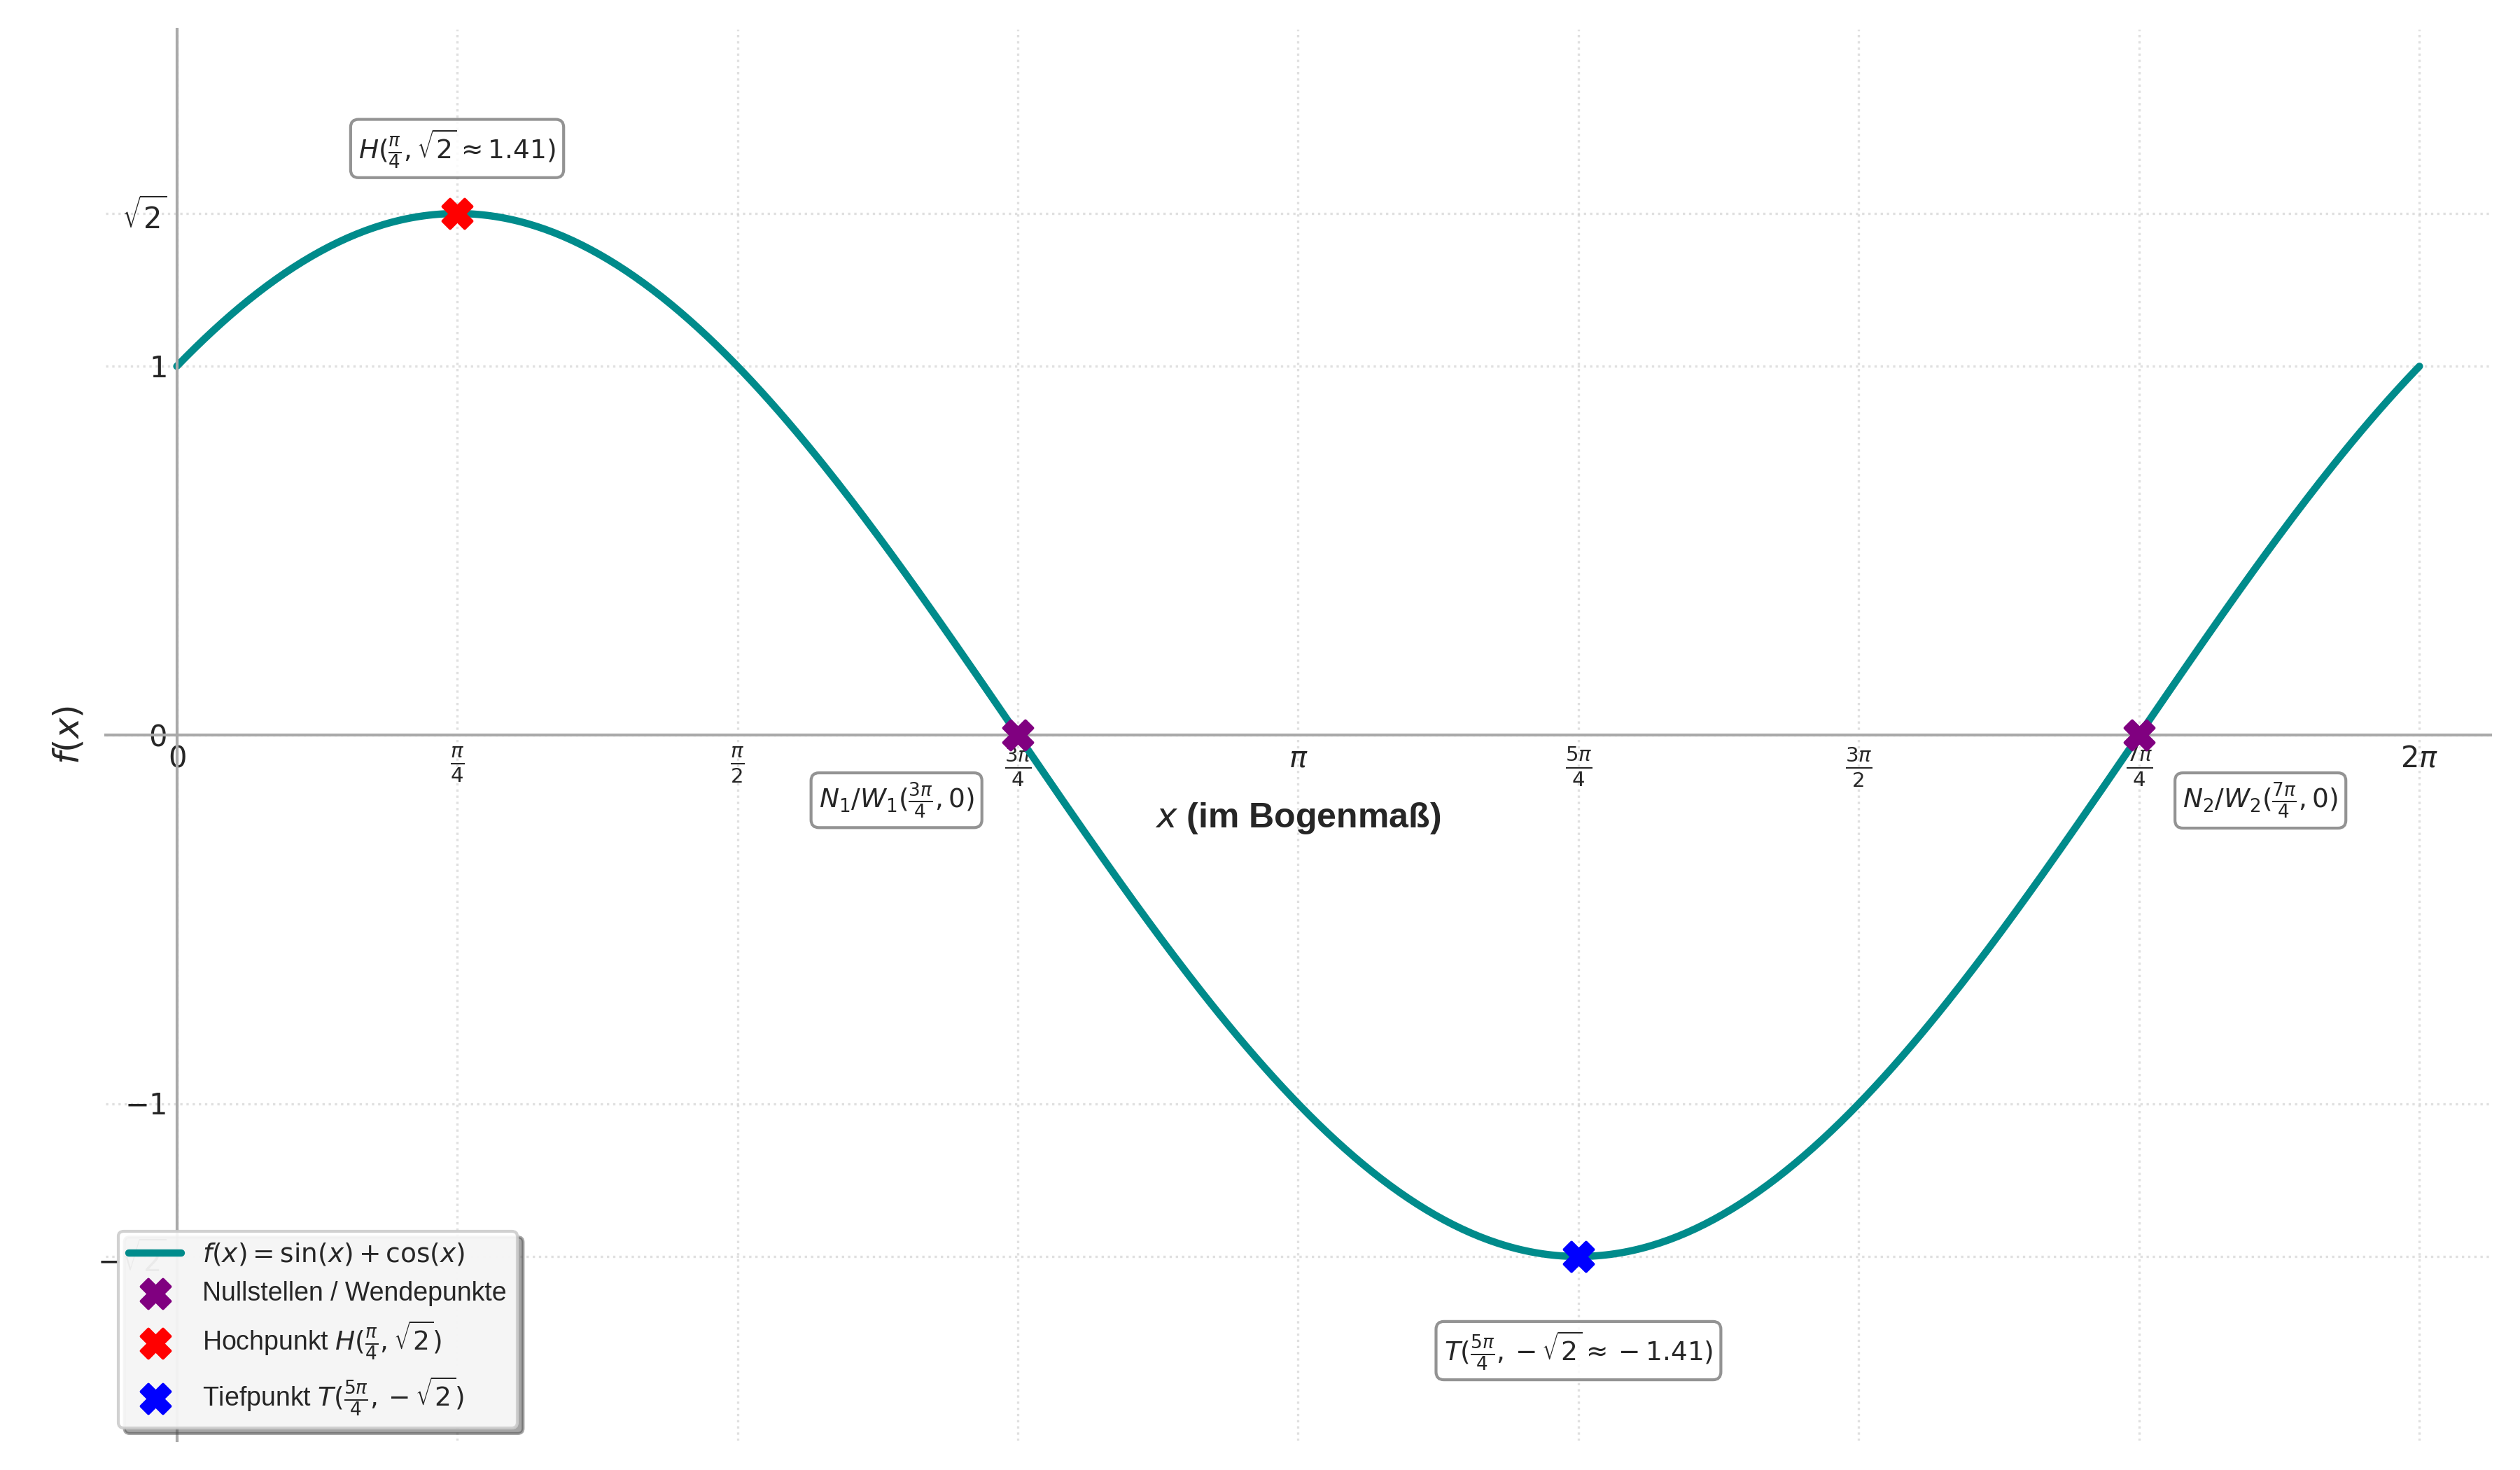
\includegraphics[width=0.9\textwidth]{grafiken/Trig_Kurvendiskussion_SinPlusCos.png}
            \captionof{figure}{Graph von $f(x)=\sin(x)+\cos(x)$}
            \label{fig:kurvendisk_sinpluscos}
        \end{center}
\end{enumerate}
\end{beispielumgebung}

\begin{aufgabenumgebung}{Kurvendiskussionen mit trigonometrischen Funktionen}
Führe eine möglichst vollständige Kurvendiskussion für die folgenden Funktionen im angegebenen Intervall durch und skizziere den Graphen. Bestimme alle Eigenschaften (Definitionsbereich, Symmetrie, Verhalten an den Rändern, y-Achsenabschnitt, Ableitungen, Monotonie, Krümmung) analytisch, soweit dies mit den dir bekannten Methoden möglich ist. 

Für Nullstellen oder die x-Koordinaten von Extrem- und Wendepunkten, deren exakte Berechnung auf \textbf{transzendente Gleichungen} führt (Gleichungen, die algebraisch nicht einfach nach der Variablen aufgelöst werden können, z.B. wenn $x$ sowohl innerhalb als auch außerhalb einer trigonometrischen Funktion steht), ist eine exakte algebraische Lösung oft nicht das Ziel.
\begin{itemize}
    \item Versuche in solchen Fällen, die \textit{Existenz} von Lösungen durch Überlegungen (z.B. Zwischenwertsatz, falls bekannt, oder Monotonie) zu begründen oder zumindest plausibel zu machen.
    \item Du kannst dann \textbf{digitale Werkzeuge} (wie Wolfram Alpha, GeoGebra oder einen grafikfähigen Taschenrechner) verwenden, um Näherungswerte für diese speziellen x-Werte zu ermitteln. Notiere in deiner Lösung, wenn du solche Näherungswerte verwendest, um deine Skizze zu vervollständigen und die Analyse abzurunden.
\end{itemize}
Der Schwerpunkt liegt auf dem Verständnis der analytischen Schritte und der Interpretation der Ergebnisse.

\begin{enumerate}
    \item $f(x) = 2\sin(x) - x$ im Intervall $[0, 2\pi]$.
        \begin{tippumgebung}{Umgang mit Nullstellen von $f(x)$}
        Du wirst feststellen, dass $x=0$ eine Nullstelle ist. Die Gleichung $2\sin(x) = x$ für weitere Nullstellen ist transzendent. Du kannst grafisch argumentieren, dass es eine weitere Nullstelle im Intervall gibt (z.B. indem du $y=2\sin x$ und $y=x$ vergleichst) oder deren ungefähre Lage mit einem digitalen Werkzeug bestimmen. Konzentriere dich ansonsten auf die exakte Berechnung der Ableitungen, Extrem- und Wendestellen, soweit möglich.
        \end{tippumgebung}
    \item $g(x) = x \cdot \cos(x)$ im Intervall $[-\pi, \pi]$.
        \begin{tippumgebung}{Umgang mit Extremstellen von $g(x)$}
        Die Nullstellen von $g(x)$ sind exakt bestimmbar. Die notwendige Bedingung für Extremstellen ($g'(x)=0$) führt hier jedoch auf die transzendente Gleichung $\cos(x) = x\sin(x)$. Untersuche die Ableitung $g'(x)$ an markanten Punkten (z.B. Nullstellen von $g(x)$ oder Ränder des Intervalls), um Bereiche mit unterschiedlichem Monotonieverhalten zu identifizieren. Für die genaue Lage der Extremstellen kannst du Näherungswerte aus digitalen Werkzeugen verwenden und dies vermerken.
        \end{tippumgebung}
\end{enumerate}
\end{aufgabenumgebung}

% \begin{kurzknappumgebung}{Trigonometrische Funktionen – Analysis}
% \begin{itemize}
%     \item \textbf{Bogenmaß} ist Standard für die Analysis.
%     \item \textbf{Ableitungen:} $(\sin x)' = \cos x$, $(\cos x)' = -\sin x$, $(\tan x)' = \frac{1}{\cos^2 x}$.
%     \item \textbf{Stammfunktionen:} $\int \sin x \,dx = -\cos x + C$, $\int \cos x \,dx = \sin x + C$.
%     \item \textbf{Transformationen $A \sin(B(x-C))+D$:} Amplitude $|A|$, Periode $P=\frac{2\pi}{|B|}$, Verschiebung $C$ (x-Richtung), $D$ (y-Richtung).
%     \item \textbf{Kettenregel} ist entscheidend für verkettete trigonometrische Funktionen (z.B. $\sin(kx)$ oder $\cos(x^2)$).
%     \item \textbf{Produkt- und Quotientenregel} für Kombinationen mit anderen Funktionen (z.B. $x \sin x$ oder $\frac{\sin x}{x}$).
%     \item \textbf{Kurvendiskussion} folgt den bekannten Schritten, Periodizität und Symmetrie sind oft hilfreich.
% \end{itemize}
% \end{kurzknappumgebung}



% Dieser Block sollte am ENDE des Kapitels zu den trigonometrischen Funktionen eingefügt werden,
% bevor das allgemeine Abschlusskapitel des gesamten Dokuments beginnt.

% Annahme: Der Hauptteil des Kapitels zu trigonometrischen Funktionen wurde bereits behandelt
% (Definitionen, Eigenschaften, Ableitungen, Stammfunktionen, Kurvendiskussionen von sin, cos, tan etc.)

\begin{kurzknappumgebung}{Trigonometrische Funktionen – Das Wichtigste im Überblick}
\begin{itemize}
    \item \textbf{Grundfunktionen:} $\sin(x)$, $\cos(x)$, $\tan(x) = \frac{\sin(x)}{\cos(x)}$.
    \item \textbf{Bogenmaß:} Standard für Winkelangaben in der Analysis ($2\pi \widehat{=} 360^\circ$).
    \item \textbf{Eigenschaften $\sin(x), \cos(x)$:}
        \begin{itemize}
            \item Definitionsbereich: $\mathbb{R}$. Wertebereich: $[-1, 1]$.
            \item Periode: $2\pi$.
            \item Nullstellen: $\sin(x)=0$ für $x=k\pi$; $\cos(x)=0$ für $x=\frac{\pi}{2}+k\pi$.
            \item Symmetrie: $\sin(x)$ ist punktsymmetrisch zum Ursprung, $\cos(x)$ ist achsensymmetrisch zur y-Achse.
            \item Trigonometrischer Pythagoras: $\sin^2(x) + \cos^2(x) = 1$.
        \end{itemize}
    \item \textbf{Eigenschaften $\tan(x)$:}
        \begin{itemize}
            \item Definitionsbereich: $\mathbb{R} \setminus \{ \frac{\pi}{2} + k\pi \}$. Polstellen bei $x = \frac{\pi}{2} + k\pi$.
            \item Wertebereich: $\mathbb{R}$. Periode: $\pi$.
            \item Nullstellen: $x=k\pi$. Punktsymmetrisch zum Ursprung.
        \end{itemize}
    \item \textbf{Wichtige Ableitungen:}
        \begin{itemize}
            \item $(\sin x)' = \cos x$
            \item $(\cos x)' = -\sin x$
            \item $(\tan x)' = \frac{1}{\cos^2 x} = 1 + \tan^2 x$
        \end{itemize}
    \item \textbf{Wichtige Stammfunktionen:}
        \begin{itemize}
            \item $\int \sin x \,dx = -\cos x + C$
            \item $\int \cos x \,dx = \sin x + C$
            \item $\int \frac{1}{\cos^2 x} \,dx = \tan x + C$ (seltener benötigt)
        \end{itemize}
    \item \textbf{Transformationen:} Funktionen der Form $A \cdot \sin(B(x-C)) + D$ beschreiben allgemeine Sinusschwingungen mit Amplitude $|A|$, Periode $P=\frac{2\pi}{|B|}$, Phasenverschiebung $C$ und Mittellage $D$.
    \item \textbf{Anwendungen:} Modellierung von periodischen Vorgängen, Schwingungen, Wellen.
\end{itemize}
\end{kurzknappumgebung}

\begin{aufgabenumgebung}{Integrationsregeln im Mix}
Nachdem du nun vielfältige Funktionen und Integrationstechniken kennengelernt hast, soll diese Aufgabe dein Verständnis und deine Fertigkeiten bei der Kombination verschiedener Regeln prüfen.

Berechne die folgenden unbestimmten Integrale. Gib an, welche Methode(n) (z.B. partielle Integration, Substitution, Grundintegrale) du verwendest.
\begin{enumerate}[label=(\alph*)]
    \item $\int x^2 \cos(x) \,dx$
        \begin{tippumgebung}{Mehrfache partielle Integration}
        Hier ist die partielle Integration zweimal anzuwenden, ähnlich wie bei $\int x^2 e^x \,dx$. Wähle den Polynomteil zum Ableiten.
        \end{tippumgebung}
    \item $\int \sin(x) \cdot e^{\cos(x)} \,dx$
        \begin{tippumgebung}{Substitution mit $e$-Funktion}
        Erkennst du eine innere Funktion $g(x)$, deren Ableitung $g'(x)$ (oder ein Vielfaches davon) ebenfalls im Integranden vorkommt? Denke an die Ableitung des Exponenten.
        \end{tippumgebung}
    \item $\int e^{2x} \cos(x) \,dx$
        \begin{tippumgebung}{Der 'Trick-Integral' mit Varianten}
        Diese Aufgabe ähnelt dem Integral $\int e^x \sin(x) \,dx$. Du wirst zweimal partiell integrieren müssen, bevor das ursprüngliche Integral (oder ein Vielfaches davon) wieder auf der rechten Seite erscheint und du die Gleichung danach auflösen kannst.
        \end{tippumgebung}
    \item \textbf{Für Experten:} $\int \sin(\ln x) \,dx$
        \begin{tippumgebung}{Knifflige Kombination}
        Versuche zuerst eine Substitution $u = \ln x$, woraus $x = e^u$ und $dx = e^u du$ folgt. Das führt zu einem Integral der Form $\int \sin(u) e^u du$, das du bereits aus einer früheren Herausforderung (Aufgabe 7.12, Teil f) kennst oder mit der dort beschriebenen Methode lösen kannst. Vergiss am Ende die Rücksubstitution nicht!
        \end{tippumgebung}
    \item \textbf{Flächenberechnung (Herausforderung):} Bestimme den Inhalt der Fläche, die vom Graphen der Funktion $f(x) = e^x \sin(x)$ und der x-Achse im Intervall $[0, \pi]$ eingeschlossen wird. Fertige eine Skizze an. Du benötigst die Stammfunktion aus Aufgabe (c) (oder der früheren Herausforderung). Beachte, dass $\sin(x)$ im Intervall $[0,\pi]$ nicht negativ ist.
\end{enumerate}
Diese Aufgaben erfordern sorgfältiges Anwenden der Regeln und oft auch mehrere Schritte. Viel Erfolg!
\end{aufgabenumgebung}





\begin{infoboxumgebung}{Die Welt der Wellen und Kreise – Ein Nachklang zu den trigonometrischen Funktionen}
Mit den trigonometrischen Funktionen hast du die mathematischen Werkzeuge kennengelernt, um die vielfältigen periodischen Rhythmen und zyklischen Muster zu beschreiben, die uns in der Natur und Technik überall begegnen – von den harmonischen Schwingungen einer gestimmten Saite über die Wellen des Lichts bis hin zu den komplexen Überlagerungen von Signalen in der Kommunikationstechnik.

Die Eleganz, mit der Sinus und Kosinus Kreisbewegungen und periodische Phänomene erfassen, ist ein weiteres wunderbares Beispiel für die tiefe Verbindung zwischen Geometrie und Analysis. Die Untersuchung ihrer Ableitungen und Integrale hat dir gezeigt, wie die Werkzeuge der Analysis auch auf diese speziellen Funktionen angewendet werden können, um ihr Verhalten genau zu verstehen und Vorhersagen zu treffen.

Vielleicht hast du bei der Beschäftigung mit Sinus und Kosinus auch schon eine Ahnung von noch tieferen Zusammenhängen bekommen, wie beispielsweise der Eulerschen Formel ($e^{ix} = \cos x + i \sin x$). Diese verblüffende Gleichung schlägt eine Brücke zwischen der Welt der Exponentialfunktionen (mit der Basis $e$) und der Welt der Trigonometrie und öffnet gleichzeitig die Tür zum Reich der komplexen Zahlen – ein weiteres faszinierendes Feld der Mathematik.

Die Reise in die Welt der Schwingungen, Wellen und periodischen Muster ist voller Entdeckungen und zeigt eindrücklich, wie universell und mächtig die Sprache der Mathematik ist, um die Phänomene um uns herum zu beschreiben und zu verstehen.
\end{infoboxumgebung}




\begin{aufgabenumgebung}{Checkliste: Bogenmaß, Einheitskreis und Grundeigenschaften verstehen}
Die Basis der trigonometrischen Funktionen liegt im Einheitskreis und der Verwendung des Bogenmaßes. Überprüfe dein Verständnis:

\begin{enumerate}[label=(\alph*)]
    \item \textbf{Bogenmaß vs. Gradmaß:}
    \begin{itemize}
        \item Erkläre mit eigenen Worten, was das Bogenmaß eines Winkels darstellt. Warum ist $180^\circ = \pi \text{ rad}$?
        \item Warum ist es in der Analysis (insbesondere beim Ableiten) wichtig, Winkel im Bogenmaß anzugeben? (Tipp: Denke an die Einfachheit der Ableitungsformeln.)
    \end{itemize}
    \item \textbf{Sinus und Kosinus am Einheitskreis:}
    \begin{itemize}
        \item Wie hängen die Koordinaten eines Punktes $P(x_P|y_P)$ auf dem Einheitskreis mit $\sin(\alpha)$ und $\cos(\alpha)$ zusammen, wenn $\alpha$ der Winkel zwischen der positiven x-Achse und dem Strahl zum Punkt $P$ ist?
        \item Erkläre mithilfe des Einheitskreises, warum der Wertebereich von $\sin(x)$ und $\cos(x)$ das Intervall $[-1, 1]$ ist.
        \item Leite die Identität $\sin^2(x) + \cos^2(x) = 1$ (Trigonometrischer Pythagoras) aus der Definition am Einheitskreis her.
    \end{itemize}
    \item \textbf{Periodizität und Symmetrie:}
    \begin{itemize}
        \item Was bedeutet es, dass $\sin(x)$ und $\cos(x)$ periodisch mit der Periode $2\pi$ sind? Wie zeigt sich das am Einheitskreis und im Graphen?
        \item Erkläre die Punktsymmetrie von $\sin(x)$ zum Ursprung ($\sin(-x)=-\sin x$) und die Achsensymmetrie von $\cos(x)$ zur y-Achse ($\cos(-x)=\cos x$) anhand des Einheitskreises.
    \end{itemize}
\end{enumerate}
\end{aufgabenumgebung}

\begin{aufgabenumgebung}{Checkliste: Transformationen und Analysis trigonometrischer Funktionen}
Die Grundfunktionen $\sin(x)$ und $\cos(x)$ können transformiert und mit den Werkzeugen der Differential- und Integralrechnung analysiert werden.

\begin{enumerate}[label=(\alph*)]
    \item \textbf{Transformierte Sinusfunktion $f(x) = A \sin(B(x-C)) + D$:}
    \begin{itemize}
        \item Wenn du eine Schwingung modellieren möchtest, die doppelt so hoch ausschlägt wie $\sin(x)$ und nur halb so schnell schwingt (also die doppelte Periode hat), wie müsstest du $A$ und $B$ wählen (angenommen $A>0, B>0$)?
        \item Wie verschiebt sich der 'Standard-Startpunkt' (der bei $\sin(x)$ im Ursprung mit positiver Steigung liegt) durch die Parameter $C$ und $D$? Was ist die Gleichung der Mittellage?
    \end{itemize}
    \item \textbf{Ableitungen und ihre Bedeutung:}
    \begin{itemize}
        \item Es gilt $(\sin x)' = \cos x$. Betrachte die Graphen von $\sin x$ und $\cos x$: An welchen Stellen hat $\sin x$ seine Extrempunkte (Hoch-/Tiefpunkte)? Was ist an diesen Stellen der Wert von $\cos x$ (also der Ableitung)? Passt das zur Regel, dass die Ableitung an Extremstellen Null ist?
        \item Umgekehrt: Wo hat $\cos x$ seine Nullstellen? Was für Punkte (bezüglich Steigung) hat $\sin x$ an diesen Stellen?
        \item Warum ist das Vorzeichen bei $(\cos x)' = -\sin x$ negativ? Versuche, dies anhand der Steigung des Kosinusgraphen zu erklären, wenn $\sin x$ positiv ist.
    \end{itemize}
    \item \textbf{Integration und Fläche:}
    \begin{itemize}
        \item Das bestimmte Integral $\int_0^{2\pi} \cos(x) \,dx = 0$. Erkläre dieses Ergebnis geometrisch anhand des Graphen von $\cos(x)$ und dem Konzept der orientierten Fläche.
        \item Wie würdest du vorgehen, um den \textit{gesamten geometrischen Flächeninhalt} zu berechnen, den der Graph von $f(x)=\sin(x)$ mit der x-Achse im Intervall $[0, 2\pi]$ einschließt? (Tipp: Nullstellen und Beträge).
    \end{itemize}
    \item \textbf{Tangensfunktion:}
    \begin{itemize}
        \item Warum ist die Tangensfunktion $\tan(x) = \frac{\sin x}{\cos x}$ nicht für alle $x \in \mathbb{R}$ definiert? Was befindet sich an den Definitionslücken im Graphen?
        \item Die Ableitung von $\tan x$ ist $(\tan x)' = \frac{1}{\cos^2 x}$. Ist diese Ableitung jemals negativ? Was bedeutet das für die Monotonie der Tangensfunktion in ihren Definitionsintervallen?
    \end{itemize}
\end{enumerate}
\end{aufgabenumgebung}


